%&LaTeX
\documentclass{article}
\usepackage{graphicx}
\usepackage{longtable}
\usepackage{url}                % For email addresses, hypertext links, ...
\DeclareGraphicsExtensions{.pdf}
\DeclareGraphicsExtensions{.eps}

\oddsidemargin 0.5in    %   Note that \oddsidemargin = \evensidemargin
\evensidemargin 0.5in
\marginparwidth 40pt      
\marginparsep 20pt      % Horizontal space between outer margin and
                % marginal note
\textwidth 5.5in        % width of text

% VERTICAL SPACING:
% Top of page:
%\topmargin .5in     %    distance from top of page to running head
\headheight 14pt     %    Height of box containing running head.
\headsep .4in        %    Space between running head and text.
\textheight 8.8in    %    space for text
\footskip 30pt       %    Distance from baseline of box containing foot
             %    to baseline of last line of text.
                                                  
\begin{document}

\vspace{-5in}
\hspace{-1in}
\vspace{-5in}
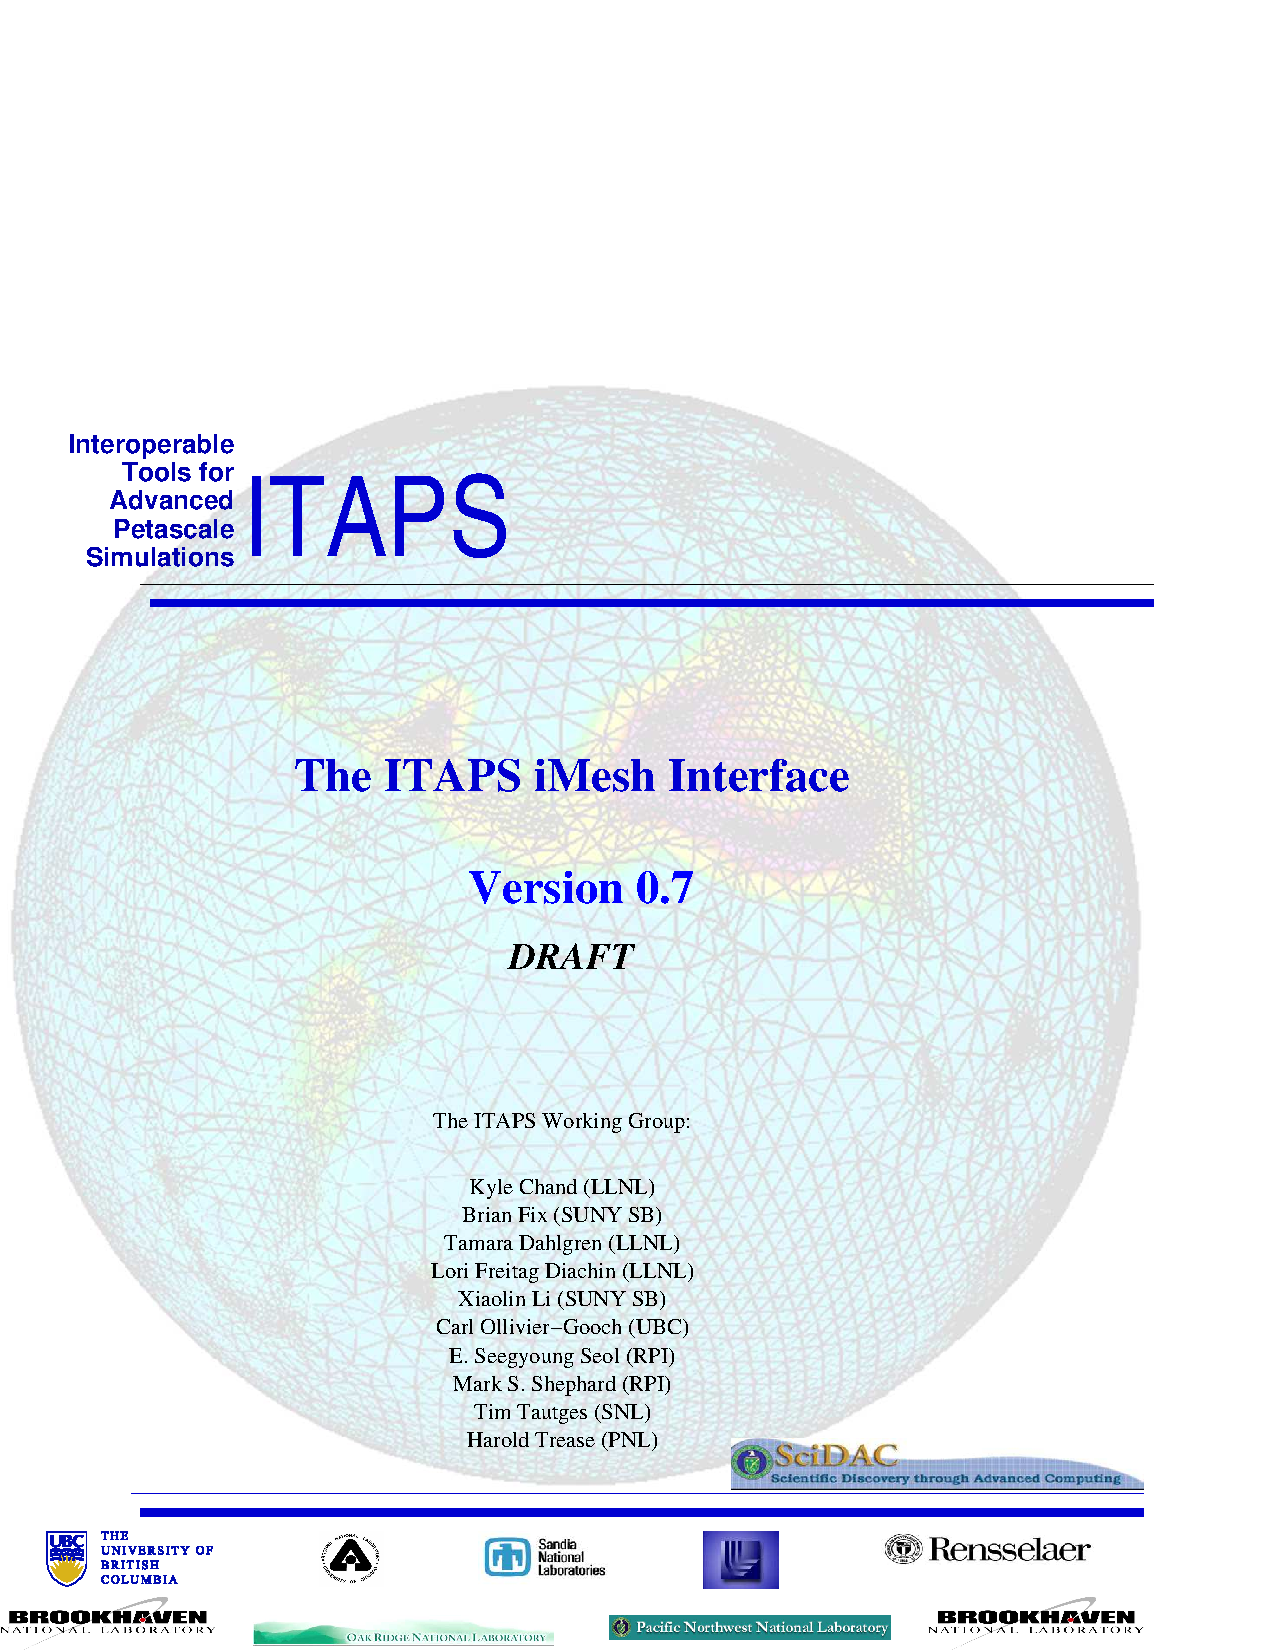
\includegraphics[height=8.5in, width=7.3in]{figures/iMesh.pdf}

\newpage
\tableofcontents
\newpage

%%%%%%%%%%%%%%%%%%%%%%%%%%%%%%%%%%%%%%%%%%%%%%%%%%%%%%%%%%
%%%%%%%%%%%%%%%%%%%%%%%%%%%%%%%%%%%%%%%%%%%%%%%%%%%%%%%%%%
\section{Introduction: Interoperability and Interchangeablity}
%%%%%%%%%%%%%%%%%%%%%%%%%%%%%%%%%%%%%%%%%%%%%%%%%%%%%%%%%%
%%%%%%%%%%%%%%%%%%%%%%%%%%%%%%%%%%%%%%%%%%%%%%%%%%%%%%%%%%

One of the primary goals of the Terascale Simulation Tools and 
Technologies (ITAPS) center is to provide an array of advanced 
meshing and discretization services to application scientists. 
These can range from mesh-based services such as mesh quality 
improvement and adaptive loop insertion to field data services 
such as high-order discretization libraries and simulation coupling 
approaches for multiscale and multiphysics applications. Ideally 
these services will be both \emph{interchangeable}, allowing experimentation 
horizontally across a number of different tools that provide 
similar functionality, and \emph{interoperable}, allowing vertical 
integration of multiple tools into a single simulation. Unfortunately, 
most modern meshing and discretization technologies are not interchangeable 
or interoperable making it difficult and time consuming for an 
application scientist to pursue a number of advanced solution 
strategies. \\

To create a set of interoperable and interchangeable services, 
the ITAPS center has defined a framework that abstracts the information 
flow in PDE-based simulations. A simulation's information flow 
begins with a problem definition. Described in more detail in 
the iGeom users' guide, the problem definition consists of a 
description of the simulation's geometric and temporal domain 
annotated by attributes designating mathematical model details 
and parameters. The description of the computational domain which 
can take one of many different forms including CAD models, image 
data, or a surface mesh. We note that the geometry can be decomposed 
into one or more subpieces if a multiphysics solution is to be 
pursued in which different mesh types or physics models are desired 
for different parts of the domain. In the next stage of the information 
flow, mesh-based simulation procedures approximate the PDEs by 
first decomposing the geometric domain into a set of piecewise 
components, \emph{the mesh}, and then approximating the continuous 
PDEs on that mesh using, for example, finite difference, finite 
volume, finite element, or partition of unity methods. These 
may be single meshes with a consistent element type or hybrid 
meshes in which multiple meshing strategies have been employed. 
All meshes at this level refer back to a single high level description 
of the computational domain (even if it has been decomposed) 
so that changes to the computational domain propagate throughout 
all associated simulation processes. The mesh can be further 
subdivided, perhaps into the components of a hybrid mesh or partitions 
across the processors of a parallel computer. In addition to 
the mesh and geometry data, the third core data type in the ITAPS 
data hierarchy is the field data or degrees of freedom used in 
the numerical solution of PDE-based applications. Once the domain 
and PDE are discretized, a number of different methods can be 
used to solve the discrete equations and visualize or otherwise 
interrogate the results. Simulation automation and reliability 
often imply feedback of the PDE discretization information back 
to the domain discretization (i.e. in adaptive methods) or even 
modification of the physical domain or attributes (e.g., design 
optimization). ITAPS uses the information flow through a mesh-based 
simulation as a framework for developing interoperable geometry, 
mesh and solution field components. While the information flow 
is modeled using the requirements of a mesh-based PDE solver, 
the resulting components are general enough to provide the infrastructure 
for a variety of other tools including pre/post-processing of 
discrete data, mesh and geometry manipulation, and error estimation.

\begin{figure}[htb] 
\begin{center}
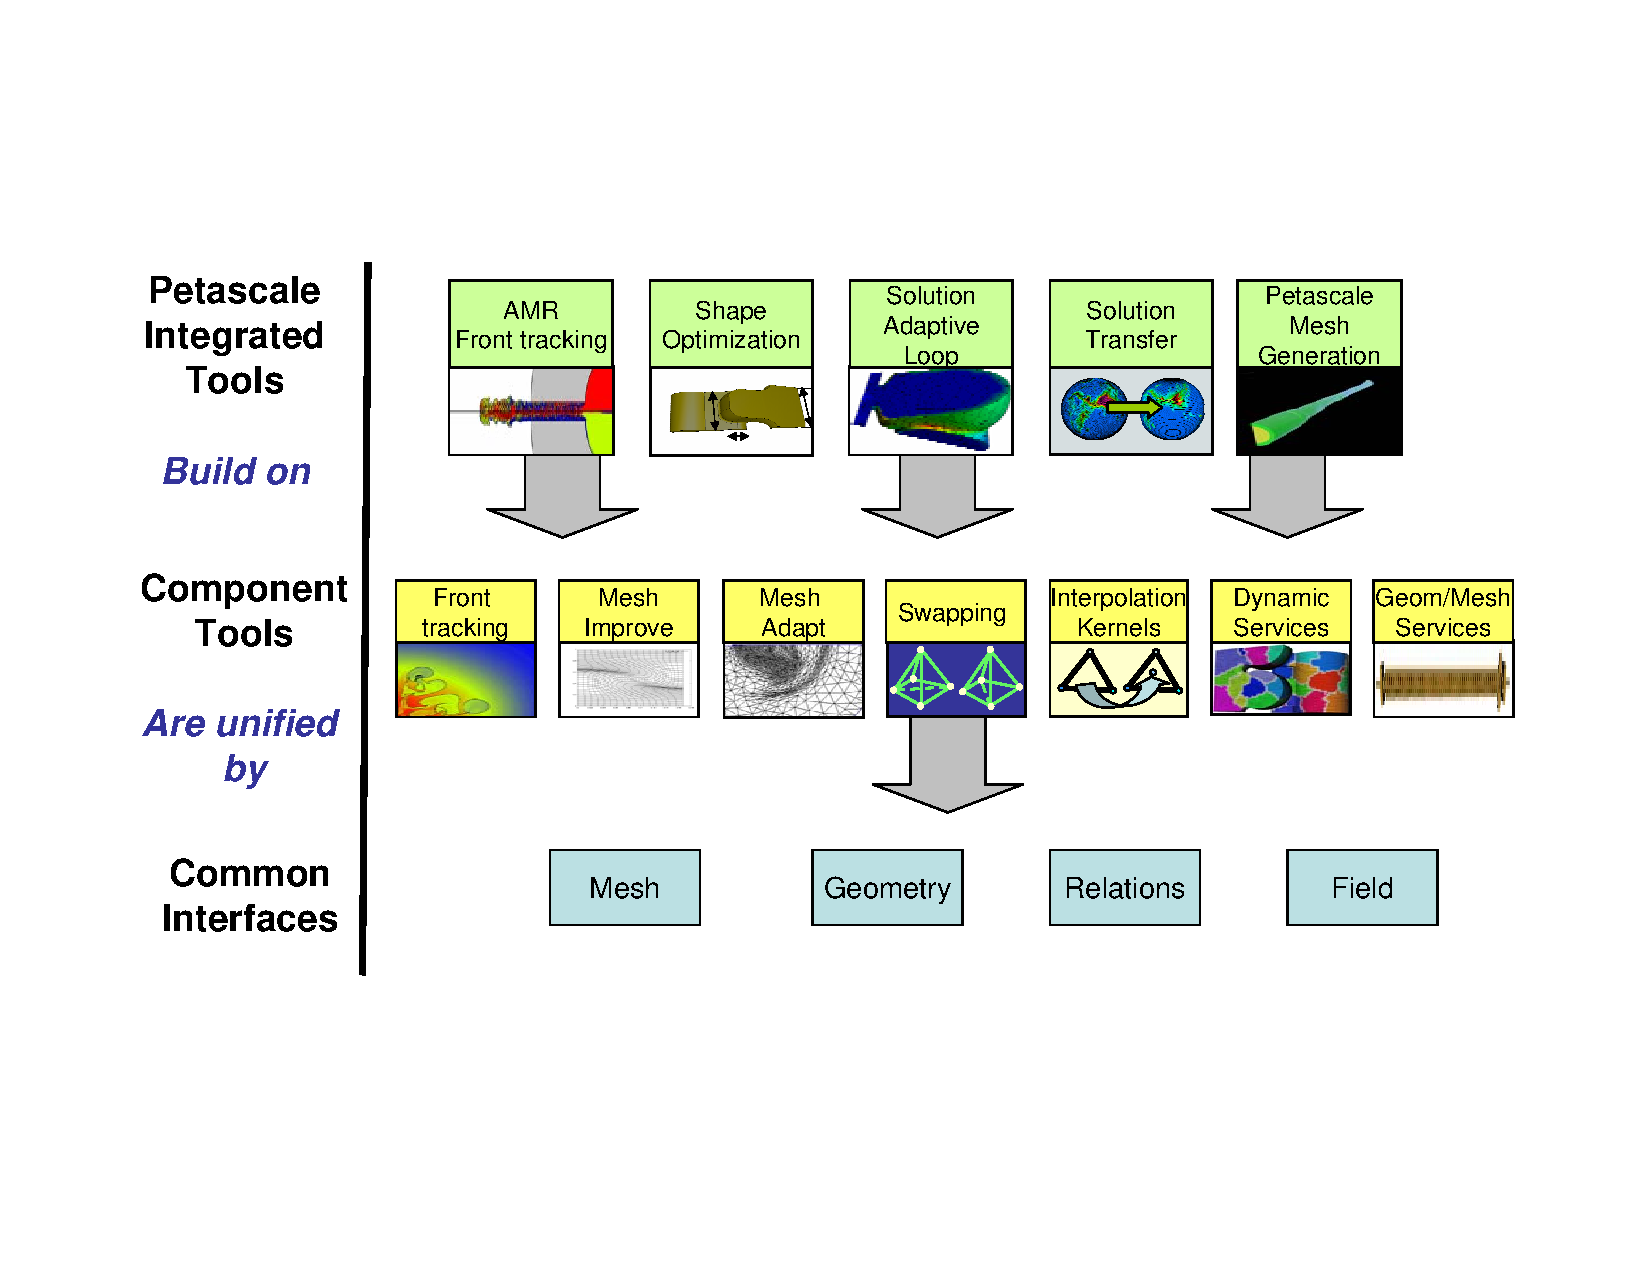
\includegraphics[angle=270,clip=true,viewport=1in .5in 7.5in 11in,width=6.5in]{figures/big-picture.pdf}
\end{center}
\vspace{-4\baselineskip}
\caption{The ITAPS center is
developing integrated services that build on multiple
component services and common interfaces for geometry, mesh and field
information.}
\label{fig:big_picture}
\end{figure}

The goal of the Interoperable Technologies for Advanced Petascale
Simulations (ITAPS) enabling technology center is to address this
challenge through the development of interoperable and interchangeable
mesh, geometry, and field manipulation tools that are of direct use to
SciDAC applications.  The hierachical approach we take to our
technology development goals is summarized in Figure
\ref{fig:big_picture}.  We start with component services
such as mesh quality improvement, adaptive loops, front tracking at
the middle level of the figure.  These services are of direct use to
applications as stand-alone tools, and many of them pre-date
the ITAPS project.  However, to use these tools in concert to form
higher-level integrated services, such as AMR-front tracking or shape
optimization (top row of the figure), application scientists must
often provide multiple interfaces to the same data which is a costly
and error prone process.  To address this problem, the ITAPS team is
developing common interfaces that provide data-structure and
implementation neutral access to mesh, geometry, and field
information.  These interfaces provide access to all ITAPS services in
a uniform way and are fundamental to creating interoperability for the
integrated services.  Moreover, a uniform interface allows easier
experimentation with different, but functionally similar, technologies
to determine which is best suited for a given application.\\

A key aspect of our approach is that we do not enforce any particular 
data structure or implementation with our interfaces, only that 
certain questions about the mesh, geometry or field data can 
be answered through calls to the interface. The challenges inherent 
in this type of effort include balancing performance of the interface 
with the flexibility needed to support a wide variety of mesh 
types. Further challenges arise when considering the support 
of many different scientific programming languages. This aspect 
is addressed through our joint work with the Center for Component 
Technologies for Terascale Simulation Science (CCTTSS) to provide 
language independent interfaces by using their SIDL/Babel technology. \\

This document focuses on the definition of the functional interface 
for ITAPS mesh data.  The interfaces defined in this document 
rely on the error, tag, and set services defined in the ITAPS 
Base interface (iBase). A portion of that documentation is included 
as an appendix here; more complete information can be found on 
the ITAPS web site. Documentation on the geometry and field data 
interfaces can be found in separate documents on the ITAPS web 
site. The remainder of this users' guide is organized as follows. 
In Section 2, we describe a number of the services the ITAPS center 
is providing that build on the mesh interface. This gives the 
reader an idea of the breadth of functionality the interface 
needs to provide. We then discuss the ITAPS mesh data model in 
Section 3, and the assumptions and conventions used in the interface 
definition process in Section 4. A functional description of 
the interface is given in Section 5 and the expected error behavior 
is summarized in Section 6. Sections 7 and 8 give examples and 
best practices guidelines that provide insight into the usage 
of the ITAPS interface. Finally, we give the current status of 
a number of different implementations and information on how 
to download and build the software in Section 9.

%%%%%%%%%%%%%%%%%%%%%%%%%%%%%%%%%%%%%%%%%%%%%%%%%%%%%%%%%%
%%%%%%%%%%%%%%%%%%%%%%%%%%%%%%%%%%%%%%%%%%%%%%%%%%%%%%%%%%
\section{ITAPS Services using the mesh interface}
%%%%%%%%%%%%%%%%%%%%%%%%%%%%%%%%%%%%%%%%%%%%%%%%%%%%%%%%%%
%%%%%%%%%%%%%%%%%%%%%%%%%%%%%%%%%%%%%%%%%%%%%%%%%%%%%%%%%%

%%%%%%%%%%%%%%%%%%%%%%%%%%%%%%%%%%%%%%%%%%%%%%%%%%%%%%%%%%
\subsection{Mesh Quality Improvement}
%%%%%%%%%%%%%%%%%%%%%%%%%%%%%%%%%%%%%%%%%%%%%%%%%%%%%%%%%%

Mesh quality improvement techniques can take a variety of forms 
ranging from a priori geometry improvements or a posteriori solution-based 
improvements. The operations that may be performed on the mesh 
include vertex movement strategies, topology modifications such 
as edge or face swapping, and h-refinement in which new elements 
are added to the mesh to improve resolution in areas where the 
error is high. The ITAPS center is supporting the development 
of a stand-alone mesh quality improvement toolkit, called Mesquite, 
which will provide state-of-the-art algorithms for vertex relocation 
and topology modification. It is designed to be flexible enough 
to work on a wide array of mesh types ranging from structured 
meshes to unstructured and hybrid meshes and a number of different 
two- and three- dimensional element types. \\

To achieve the maximum amount of improvement in the mesh, vertex 
relocation schemes must be able to operate both on the surface 
of the geometric domain as well as in the interior volume. This 
implies that the software must have functional access to both 
the high level description of the geometric domain as well as 
to individual mesh entities such as element vertices. In particular, 
to operate on interior vertices, Mesquite must be able to query 
a ITAPS implementation for vertex coordinate information, adjacency 
information, the number of elements of a given type or topology, and 
also be able to update or change vertex coordinate information. 
To operate on the surface mesh, Mesquite must also be able to 
make a number of point-wise queries to the high-level geometry 
description for surface normal information and closest point 
information. We note that explicit classification of the mesh 
vertex against a geometric surface is required as there are some 
cases for which the closest point query will return a point on 
the wrong surface that will result in inverted or invalid meshes.\\ 


The ITAPS center is also supporting the development of a simplicial 
mesh topology modification tool, which performs face and edge 
swapping operations. This tool has been implemented using
the ITAPS mesh interface, enabling swapping in any ITAPS implementation 
supporting triangles (2D) or tetrahedra (3D). In gathering enough 
information to determine whether a swap is desirable, any mesh 
topology modification scheme must make extensive use of the ITAPS 
entity adjacency and vertex coordinate retrieval functions. Reconfiguring 
the mesh, when this is appropriate, requires deletion of old 
entities and creation of new entities through the ITAPS interface. 
In addition, classification operators are again essential. For 
instance, reconfiguring tetrahedra that are classified on different 
geometric regions results in tetrahedra that are not classified 
on either region, so this case must be avoided. Likewise, classification 
checks make it easy to identify and disallow mesh reconfigurations 
that would remove a mesh edge classified on a geometric edge.\\

In addition to basic geometry, topology and classification information, 
a ITAPS implementation must provide additional information for 
mesh improvement schemes to operate effectively and efficiently. 
For example, even for simple mesh improvement schemes, the implementation
must be able to indicate which entities may be modified and which 
may not. For mesh improvement schemes to operate on an entire 
mesh rather than simply accepting requests entity by entity, 
a ITAPS implementation must support some form of iterator. Furthermore, 
advanced schemes may allow the user to input a desired size, 
orientation, degree of anisotropy, or even an initial reference 
mesh; exploiting such features will require the implementation 
to associate many different types of information with mesh entities 
and pass that information to the mesh improvement scheme when 
requested.

%%%%%%%%%%%%%%%%%%%%%%%%%%%%%%%%%%%%%%%%%%%%%%%%%%%%%%%%%%
\subsection{Adaptive Loop Insertion}
%%%%%%%%%%%%%%%%%%%%%%%%%%%%%%%%%%%%%%%%%%%%%%%%%%%%%%%%%%

A great number of codes have been developed for the solution 
of partial differential equations. Increasingly the users of 
these codes are requesting that they include support for adaptive 
discretization error control. One approach to support the application 
of adaptive analysis is to alter the analysis code to include the error estimation and mesh 
adaptation methods needed. The advantage of this approach is 
that the resulting code can minimize the total computation and 
data manipulation time required. The disadvantage is the amount of 
code modification and development required to support mesh adaptation 
is extensive since it requires extending the data structures 
and all the procedures that interact with them. The expense and 
time required to do this for existing fixed mesh codes is large 
and, in most cases, considered prohibitive. \\


The alternative approach is to leave the fixed mesh analysis 
code unaltered and to use the interoperable mesh, geometry and 
field components to control the flow of information between the 
analysis code and a set of other needed components. This approach 
has been used to develop multiple adaptive analysis capabilities 
in which the mesh, geometry and field components are used as 
follows.

\begin{itemize}
\item
The geometry interface supports the integration with multiple 
CAD systems. The API of the modeler enables interactions with 
mesh generation and mesh modification to obtain all domain geometry 
information needed.

\item
The mesh interface provides the services for storing and modifying 
mesh data during the adaptive process. The Algorithm-Oriented 
Mesh Database was used for the examples given here.

\item
The field interface provides the functions to obtain the solution 
information needed for error estimation and to support the transfer 
of solution fields as the mesh is adapted.
\end{itemize}


One approach to support mesh adaptation is to use error estimators 
to define a new mesh size field that is provided to an automatic 
mesh generator that creates an entirely new mesh of the domain. 
Although a popular approach, it has two disadvantages. The first 
is the computational cost of an entire mesh generation each time 
the mesh is adapted. The second is that in the case of transient 
and/or non-linear problems, it requires global solution field 
transfer between the old and new meshes. Such solution transfer 
is not only computationally expensive, the additional error introduced can affect 
the obtainable solution accuracy. An alternative approach to 
mesh adaptation is to apply local mesh modifications that can 
range from standard templates, to combinations of mesh modifications, 
to localized remeshing. Such procedures have been developed that 
ensure the mesh's approximation to the geometry is maintained 
as the mesh is modified. This is the approach used here.\\


Given a flexible set of adaptive control components, adaptive 
loops can and have been built for insertion into existing simulation codes. 
The adaptive loops developed can operate directly from a CAD 
geometric model domain or from a mesh model. In both cases a 
high-level topological model of the domain is used to control 
the interactions with the domain definition. Using this, in conjunction 
with mesh topology operations, meshes can be generated using 
automatic meshing procedures or adapted using a set of mesh modification 
functions that alter the mesh to match the new mesh size field. 
The field structures and functions support the construction of 
error estimators and the transfer of solution fields to the adapted 
mesh, either incrementally during mesh modification or for the 
entire mesh after mesh adaptation is complete.\\

The creation of such adaptive loops has been done for two finite 
element codes and we highlight those efforts here as examples 
of the use of ITAPS interfaces in this problem regime. The first example is 
the frequency domain electromagnetics simulation code OMEGA3P 
developed at SLAC. The second is a commercial metal forming simulation 
code where the adaptive loop tracks the evolving geometry. \\


The Stanford Linear Accelerator Center's (SLAC) eigenmode solver, 
Omega3P, is used to design of next generation linear accelerators. 
ITAPS researchers have collaborated with SLAC scientists to augment 
this code with adaptive mesh control to improve the accuracy 
and convergence of wall loss (or quality factor) calculations 
in accelerator cavities. The simulation procedure consists of 
interfacing Omega3P to solid models, automatic mesh generation,
general mesh modification, and error estimator components to 
form an adaptive loop. The accelerator geometries are defined 
as ACIS solid models. Using functional interfaces between CAD 
and meshing techniques, any number of automatic mesh generation 
tools can be used to get an initial mesh. After Omega3P calculates 
the solution fields, the error indicator determines a new mesh 
size field, and the mesh modification procedures adapt the mesh. 
The adaptive procedure has been applied to a Trispal 4-petal 
accelerator cavity. The procedure has been shown to reliably 
produce results of the desired accuracy for approximately one-third 
the number of unknowns as produced by the previous user-controlled
 procedure.\\

 Since the full accelerator models are expected to require meshes 
of up to 100 million elements the adaptive procedure must operate 
in parallel on a distributed mesh. Parallelization of the adaptive 
loop is currently under development.\\


In 3D metal forming simulations, the workpiece undergoes large 
plastic deformations that result in major changes in the domain 
geometry. The meshes of the deforming parts typically need to 
be frequently modified to continue the analysis due to large 
element distortions, mesh discretization errors and/or geometric 
approximation errors. In these cases, it is necessary to replace 
the deformed mesh with an improved mesh that is consistent with 
the current geometry. Procedures to determine a new mesh size 
field considering each of these factors have been developed and 
used in conjunction with local mesh modification. The procedure 
includes functions to transfer history dependent field variables 
as each mesh modification is performed.

%%%%%%%%%%%%%%%%%%%%%%%%%%%%%%%%%%%%%%%%%%%%%%%%%%%%%%%%%%
%%%%%%%%%%%%%%%%%%%%%%%%%%%%%%%%%%%%%%%%%%%%%%%%%%%%%%%%%%
\section{Mesh Data Model}
%%%%%%%%%%%%%%%%%%%%%%%%%%%%%%%%%%%%%%%%%%%%%%%%%%%%%%%%%%
%%%%%%%%%%%%%%%%%%%%%%%%%%%%%%%%%%%%%%%%%%%%%%%%%%%%%%%%%%

The ITAPS data models for mesh, geometry and fields all make use 
of the concepts of entities, entity sets, and tags, and we describe 
these briefly here. General information on entity sets and tags, 
along with interface specifications for their use, can be found 
in the iBase documentation.\\


ITAPS \emph{entities} are used to represent atomic pieces of information 
such as a vertices in a mesh or edges in a geometric model. To 
allow the interface to remain data structure neutral, entities 
(as well as entity sets and tags) are uniquely represented by 
32-bit opaque handles. Unless entities are added or removed, 
these handles must be invariant through different calls to the 
interface in the lifetime of the ITAPS interface, in the sense 
that a given entity will always have the same handle. Handles 
can be invariant in the face of mesh modification, but this is 
not guaranteed. \\


A ITAPS \emph{entity set} is an arbitrary collection of ITAPS entities. 
Each entity set may be an unordered set or it may be a (possibly 
non-unique) ordered list of entities. When a ITAPS interface is 
first created in a simulation, a \emph{Root Set} is created and 
can be populated using the load functionality. In addition to 
containing entities, entity sets may be related to each other 
in one of two ways.

\begin{itemize}
\item
An entity set may \emph{contain} one or more entity sets. An entity 
set contained in another may be either a subset or an element 
of that entity set. The choice between these two interpretations 
is left to the application; the ITAPS API does not discriminate 
between these interpretations. If entity set A is contained in 
entity set B, a recursive request for the contents of B will include 
the entities in A and the entities in sets contained in A; non-recursive 
and partially recursive requests are also possible.  We note that 
the \emph{Root Set} cannot be contained in another entity set.


\item
\emph{Parent/child relationships} between entity sets are used to 
represent relations between sets, much like directed edges connecting 
nodes in a graph. This relationship can be used to indicate that 
two meshes have a logical relationship to each other, including 
multigrid and adaptive mesh sequences. Because we distinguish 
between parent and child links, this is a directed graph. Also, 
the meaning of cyclic parent/child relationships is dubious, 
at best, so graphs must be acyclic. No other assumptions are 
made about the graph.
\end{itemize}

Users are able to query entity sets for their entities and entity 
adjacency relationships. Both array- and iterator-based access 
patterns are supported. In addition, entity sets also have ``set
operation'' capabilities; in particular, existing ITAPS 
entities may be added to or removed from the entity set, and 
sets may be subtracted, intersected, or united. \\

ITAPS \emph{tags} are used as containers for user-defined opaque data 
that can be attached to ITAPS entities and entity sets. Tags can 
be multi-valued which implies that a given tag handle can be 
associated with many different entities. In the general case, 
ITAPS tags do not have a predefined type and allow the user to 
attach any opaque data to ITAPS entities, each with a (potentially) 
distinct value. To improve ease of use and performance, we support 
three specialized tag types: integers, doubles, and entity handles. 
Tags have and can return their string name, size, handle and 
data. Tag data can be retrieved from ITAPS entities by handle 
in an agglomerated or individual manner. The ITAPS implementation 
is expected to allocate the memory as needed to store the tag 
data.

%%%%%%%%%%%%%%%%%%%%%%%%%%%%%%%%%%%%%%%%%%%%%%%%%%%%%%%%%%
\subsection{Mesh Entity}
%%%%%%%%%%%%%%%%%%%%%%%%%%%%%%%%%%%%%%%%%%%%%%%%%%%%%%%%%%

ITAPS \emph{mesh entities} are the fundamental building blocks of 
the ITAPS mesh interface and correspond to the individual pieces 
of the domain decomposition (mesh). Under the assumption that 
each topological mesh entity of dimension $d$, $M^d_i$, 
is bounded by a set of topological mesh entities of dimension $d-1$, 
\{$M^d_I$\{$M^{d-1}$\}\}, the full set of mesh topological entities are:
\begin{equation}
T^M = \left\{ \left\{ M \left\{ M^0 \right\} \right\}, 
             \left\{ M \left\{ M^1 \right\} \right\}, 
             \left\{ M \left\{ M^2 \right\} \right\},
	     \left\{ M \left\{ M^3 \right\} \right\} \right\}
\end{equation}
where $\left\{ M \left\{ M^d \right\} \right\}$, $d=0,1,2,3$, are respectively 
the set of vertices, edges, faces and regions which define the 
topological entities of the mesh domain. It is possible to limit 
the mesh representation to just these entities under the following 
restrictions.

\begin{itemize}
\item  
Regions and faces have no interior holes.
\item  
Each entity of order $d_i$ in a mesh, $M^{d_i}_i$, may 
use a particular entity of lower order, $d_j$, $M^{d_j}_j$, $d_j <d_i$, at most once.
\item  
For any entity $M^{d_i}_i$ there is a unique 
set of entities of order $d_i - 1$ , $\left\{ M^{d_i}_i \left\{ M^{d_i - 1} 
\right\} \right\}$ that are on the boundary of $M^{d_i}_i$.

\end{itemize}

The first restriction means that regions may be directly represented 
by the faces that bound them, faces may be represented by the 
edges that bound them, and edges may be represented by the vertices 
that bound them. The second restriction allows the orientation 
of an entity to be defined in terms of its boundary entities. 
For example, the orientation of an edge, $M^{1}_i$ bounded 
by vertices $M^{0}_j$ and $M^{0}_k$ is uniquely 
defined as going from $M^{0}_j$ to $M^{0}_k$ 
only if  $j \neq k$. The third restriction means 
that a mesh entity is uniquely specified by its bounding entities. 
Most representations including that used in the ITAPS interface 
employ that requirement. There are representational schemes where 
this condition only applies to interior entities; entities on 
the boundary of the model may have a non-unique set of boundary 
entities.\\

Specific examples of mesh entities include, for example, a hexahedron, 
tetrahedron, edge, triangle and vertex. Mesh entities are classified 
by their entity type (topological dimension) and entity topology 
(shape). Just as for geometric entities, allowable mesh entity 
types are vertex (0D), edge (1D), face (2D), and region (3D). 
Allowable entity topologies are point (0D); line segment (1D); 
triangle, quadrilateral, and polygon (2D); and tetrahedron, pyramid, 
prism, hexahedron, septahedron, and polyhedron (3D); each of 
these topologies has a unique entity type associated with it. 
Mesh entity geometry and shape information is associated with 
the individual mesh entities. For example, the vertices will 
have coordinates associated with them. Higher-dimensional mesh 
entities can also have shape information associated with them. 
For example the coordinates of higher-order finite-element nodes 
can be associated with mesh edges, faces, and regions.\\

An entity can return both upward and downward 
adjacency information (if it exists) in the canonical ordering 
using both individual and agglomerated request mechanisms. Vertices 
can return coordinate information in blocked or interleaved fashion. 
All entities have the ability to add, remove, retrieve, and set, 
user-defined tag data. 

%%%%%%%%%%%%%%%%%%%%%%%%%%%%%%%%%%%%%%%%%%%%%%%%%%%%%%%%%%
\subsection{Entity Adjacencies}
%%%%%%%%%%%%%%%%%%%%%%%%%%%%%%%%%%%%%%%%%%%%%%%%%%%%%%%%%%

Higher-dimensional entities are defined by lower-dimensional 
entities with shape and orientation defined using canonical ordering 
relationships. To determine which adjacencies are supported by 
an underlying implementation, an adjacency table is defined which 
can be returned by a query through the interface. The implementation 
can report that adjacency information is always, sometimes, or 
never available; and to be available at a cost that is constant, 
logarithmic (i.e., tree search), or linear (i.e., search over all entities) 
in the size of the mesh. The use of a table allows the implementation 
to provide separate information for each upward and downward 
adjacency request. If adjacency information exists, entities 
must be able to return information in the canonical ordering defined 
in Appendix A using both individual and agglomerated request 
mechanisms.\\


\emph{Definition:} Adjacencies describe how mesh entities connect 
to each other

\begin{itemize} 
\item  
First-order adjacencies: For an entity of dimension $d$, first-order 
adjacencies return all of the mesh entities of dimension $q$, 
which are either on the closure of the entity ($d$> $q$, \emph{downward 
adjacency}), or which it is on the closure of ($d$ <$q$, \emph{upward 
adjacency}). 
\item  
Second-order adjacencies: For an entity of dimension $d$, second-order 
adjacencies describe all of the mesh entities of dimension $q$ 
that share any adjacent entities of dimension $b$, where $d \neq b$ 
and $b \neq q$. Second-order adjacencies can be derived 
from first-order adjacencies. 
\end{itemize}


\emph{Capabilities:} In addition to downward and upward adjacency 
queries at the entity level, availability of first-order adjacencies 
and the cost for computing available adjacencies are provided 
for each ITAPS mesh implementation.\\



\emph{Examples:} For a given face, a set of regions adjacent to 
the face (first-order upward), a set of vertices bounding the 
face (first-order downward), a set of faces that share any vertex 
of the face (second-order).

%%%%%%%%%%%%%%%%%%%%%%%%%%%%%%%%%%%%%%%%%%%%%%%%%%%%%%%%%%
\subsection{Mesh Entity Sets}
%%%%%%%%%%%%%%%%%%%%%%%%%%%%%%%%%%%%%%%%%%%%%%%%%%%%%%%%%%

ITAPS \emph{mesh entity sets} are extensively used to collect mesh 
entities together in meaningful ways, for example, to represent 
the set of all faces classified on a geometric face, or the set 
of regions in a domain decomposition for parallel computing. 
For some computational applications, it is useful for entity 
sets to comprise a valid computational mesh. The simplest example 
of this is a nonoverlapping, connected set of ITAPS region entities, 
for example, the structured and unstructured meshes commonly 
used in finite element simulations. Collections of entity sets 
can compose, for example, overlapping and multiblock meshes. 
In both of these examples, supplemental information on the interactions 
of the mesh sets will be defined and maintained by the application. 
Smooth particle hydrodynamic (SPH) meshes can consist of a collection 
of ITAPS vertices with no connectivity or adjacency information.\\


Each mesh entity set may be a true set ( in the set theoretic 
sense) or it may a (possibly non-unique) ordered list of entities.  
Many entity sets may be associated with the Root Set and the entity 
set paradigm described earlier allows us to manage these entities 
and the relationships among them.  \\

\emph{Capabilities}: Mesh entity sets provide basic query capabilities 
to return entities and their adjacencies through array or iterator 
mechanisms. In addition entity sets also have ``set operation'' 
capabilities; in particular, you may add and remove existing 
ITAPS entities from the root set to the entity set and you may 
subtract, intersect, or unite entity sets. In addition, subset 
and hierarchical parent/child relationships among entity sets 
are supported. All entity sets have the ability to add, retrieve, 
and delete user-defined tag data.\\

\emph{Examples}: a set of vertices, the set of all faces classified 
on a geometric face, the set of regions in a domain decomposition 
for parallel computing, the set of all entities in a given level 
of a multigrid mesh sequence.

%%%%%%%%%%%%%%%%%%%%%%%%%%%%%%%%%%%%%%%%%%%%%%%%%%%%%%%%%%
\subsection{Modifiable Meshes}
%%%%%%%%%%%%%%%%%%%%%%%%%%%%%%%%%%%%%%%%%%%%%%%%%%%%%%%%%%

The root set can be extended to be ``modifiable'', in which case, 
basic operations that allow applications to create and destroy 
mesh entities are provided. Modifiable meshes require a minimal 
interaction with the underlying geometric model to classify entities 
and this interaction is described in the iRel document.


%%%%%%%%%%%%%%%%%%%%%%%%%%%%%%%%%%%%%%%%%%%%%%%%%%%%%%%%%%
%%%%%%%%%%%%%%%%%%%%%%%%%%%%%%%%%%%%%%%%%%%%%%%%%%%%%%%%%%
\section{Interface Definition Conventions}
%%%%%%%%%%%%%%%%%%%%%%%%%%%%%%%%%%%%%%%%%%%%%%%%%%%%%%%%%%
%%%%%%%%%%%%%%%%%%%%%%%%%%%%%%%%%%%%%%%%%%%%%%%%%%%%%%%%%%

In this document, we use \emph{application} to indicate a code that 
will use the ITAPS mesh interface, and \emph{implementation} to indicate 
a code that provides the ITAPS mesh interface.

%%%%%%%%%%%%%%%%%%%%%%%%%%%%%%%%%%%%%%%%%%%%%%%%%%%%%%%%%%
\subsection{Scientific Interface Definition Language}
%%%%%%%%%%%%%%%%%%%%%%%%%%%%%%%%%%%%%%%%%%%%%%%%%%%%%%%%%%

In the interfaces presented in this document we use the Scientific 
Interface Definition Language (SIDL) to define the functions. 
Each argument in the SIDL interface specification has both a 
type and a mode associated with it. We extensively use SIDL's 
fundamental types including bool, int, double, string, opaque, 
and enumerations.\footnote{We do not use objects due to the perceived 
cost of object creation and access at a fine grained level such 
as mesh entity by entity access. To validate this design choice, 
experiments are underway involving the ITAPS and Babel teams to 
quantify the performance differences among language specific 
bindings, SIDL bindings with opaques, and SIDL bindings with 
objects.} \\

Argument modes can be one of \emph{in, out} or \emph{inout.} In general, 
SIDL defines \emph{in} to be a parameter that is passed into the 
implementation (but is not necessarily a const), \emph{out} to be 
parameters that are passed out of the implementation, and \emph{inout} 
to be parameters that do both. For ITAPS purposes, we expect the 
following, more restrictive behavior to be associated with implementations

\begin{itemize}
\item
\emph{in}: the parameter is passed into the implementation. It is 
guaranteed that any variable passed as an `in' argument will not 
be modified within the function call, even if a particular language 
implements the function call using pass-by-reference semantics. 

\item\emph{out}: the parameter is passed out of the implementation 
and is not expected to contain meaningful data upon entering. 
The underlying implementation is free to operate as needed to 
allocate the necessary space and assign a meaningful value.

\item  \emph{inout:} the parameter is passed into the implementation 
and may or may not contain useful information upon entering the 
function. Its value can be changed by the underlying implementation. 
Arrays declared to be inout typically have `out' semantics. That 
is, any values originally contained in the array are often overwritten 
by the underlying implementation but it is passed as inout so 
storage in the array can be allocated either inside or outside 
the function call.
\end{itemize}

We use SIDL arrays and have the following general expectations 
of the interactions of the application and the implementation 
for their use as \emph{inout} arguments.
\begin{itemize}
\item  The application must allocate sufficient space in the array or 
pass an empty, unallocated array
\item  If the passed array is unallocated, the implementation will allocate 
sufficient space in the array
\item  If the passed array is allocated, the implementation will indicate 
an error condition if the allocated space is not sufficient for 
the requested data.
\item  If the passed array is allocated, it must be allocated as an 1-dimenstional 
array (a vector)
\item  If the particular language requires an explicit call to release 
the array storage, it is the responsibility of the caller to 
do so regardless of whether or not the storage was allocated 
within the function.
\item  For each array, we return the number of entries, \emph{n}, that 
contain useful information in the array. These entries are stored 
in the first \emph{n} positions of the array. This allows the array 
to be longer than is needed so that is can be used as a work 
array in many function calls rather than reinitializing a new 
array each time one is needed.
\end{itemize}


Functions that work with arrays that contain a set of fixed-length 
vectors of data (such as vertex coordinate triples) may accept 
or return such arrays ordered in either an interleaved or blocked 
manner. The application may request either order, and the implementation 
is expected to be able to provide both. It is recognized that 
the implementation may have a preferred, native storage order 
and this preferred ordering may be queried by the application.


%%%%%%%%%%%%%%%%%%%%%%%%%%%%%%%%%%%%%%%%%%%%%%%%%%%%%%%%%%
\subsection{Function Naming Conventions}
%%%%%%%%%%%%%%%%%%%%%%%%%%%%%%%%%%%%%%%%%%%%%%%%%%%%%%%%%%

ITAPS interfaces have the following naming conventions:
\begin{itemize}
\item As much as possible, functions start with a verb describing the 
action of the implementation, for example, \emph{get, set, create, 
destroy.}
\item To provide maximum flexibility for achieving performance, 
we have defined interfaces that allow access to information for 
either individual entities (\emph{single entity access)} or for 
several entities agglomerated into an array (\emph{agglomerated 
entity access)}. Functions that operate on individual entities 
contain ``Ent'' in the function name; functions that operated 
on arrays of entities contain ``Arr'' or ``EntArr''
\item Function arguments that contain the word ``handle'' 
are opaque references to underlying implementation data structures. 
The application should not make any assumptions about the specific 
value of the handle.
\item Members of enumerated types are given in capital letters

\end{itemize}

To accommodate the 31-character limit imposed by some Fortran 
compilers we have used the following abbreviations in the function 
names.
\begin{itemize}
\item {\tt Coords} for coordinates
\item {\tt Vtx} for vertex
\item {\tt Ent} for entity
\item {\tt Arr} for array
\item {\tt Adj} for adjacency
\item {\tt Dim} for dimension
\item {\tt Dflt} for default
\item {\tt Topo} for topology
\item {\tt Num} for number
\item {\tt Init} for initialize
\item {\tt Iter} for iterator
\item {\tt Chldn} for children ({\tt chld} for child)
\item {\tt Prnts} for parents ({\tt prnt} for parent)
\item {\tt Rmv} for remove
\item {\tt Int} for integer
\item {\tt Dbl} for double
\item {\tt EH} for entity handle
\end{itemize}

%%%%%%%%%%%%%%%%%%%%%%%%%%%%%%%%%%%%%%%%%%%%%%%%%%%%%%%%%%
\subsection{Tag Conventions}
%%%%%%%%%%%%%%%%%%%%%%%%%%%%%%%%%%%%%%%%%%%%%%%%%%%%%%%%%%

We have defined the following tag conventions for use with the 
ITAPS interface.\\

\begin{tabular}{llp{2.4in}}
\hline
String Name &Association  &Meaning\\
\hline
Error\_Behavior & root\_set & One of the ErrorAction enumerated types. 
 The user can change this to change the error behavior (default: THROW\_ERROR) \\
Is\_List  & entity\_set & The order of the data in the entity set has 
meaning\\

Uniquely\_Defined\_Entities &root\_set  &Does the mesh allow the 
creation and storage of duplicate entities ({\tt TRUE} indicates unique entities 
   only, {\tt FALSE} indicates the implementation can 
   handle duplicates.\\
\hline
\end{tabular}

%%%%%%%%%%%%%%%%%%%%%%%%%%%%%%%%%%%%%%%%%%%%%%%%%%%%%%%%%%
%%%%%%%%%%%%%%%%%%%%%%%%%%%%%%%%%%%%%%%%%%%%%%%%%%%%%%%%%%
\section{Mesh Interface Functionality}
%%%%%%%%%%%%%%%%%%%%%%%%%%%%%%%%%%%%%%%%%%%%%%%%%%%%%%%%%%
%%%%%%%%%%%%%%%%%%%%%%%%%%%%%%%%%%%%%%%%%%%%%%%%%%%%%%%%%%

%%%%%%%%%%%%%%%%%%%%%%%%%%%%%%%%%%%%%%%%%%%%%%%%%%%%%%%%%%
\subsection{Input/Output}
%%%%%%%%%%%%%%%%%%%%%%%%%%%%%%%%%%%%%%%%%%%%%%%%%%%%%%%%%%

ITAPS provides a basic input/output mechanism to allow the user 
to load data into the mesh data base and save any changes back 
to a file named in the input parameter list. The underlying storage 
mechanism is implementation dependent and we do not provide a 
common file format for ITAPS meshes and geometries. \\

Load information into the ITAPS mesh interface. A ``root'' entity 
set is created when the interface is created and may be accessed 
before data is loaded. Data is read into the root set and also 
into the entity set specified, if different from the root set. 
If duplicate data is read in, then duplicate data will exist 
in the root set; no attempt to merge data is made at this stage. 
For those implementations that do not support duplicate data 
an error will be returned. Tag conventions will be used to specify 
optional behavior and are defined by each individual implementation. 

\begin{verbatim}
    void load( in opaque entity_set_handle, in string name
             ) throws iBase.Error;
\end{verbatim}

Save the ITAPS entity set. Only entities explicitly contained in 
the entity set ( including subsets) are written to a file. Any 
needed adjacency information must be explicitly included in the 
set, or it will not be saved. What is saved is file format and 
implementation dependent.

\begin{verbatim}
    void save ( in opaque entity_set_handle, in string name
              ) throws iBase.Error;
\end{verbatim}


%%%%%%%%%%%%%%%%%%%%%%%%%%%%%%%%%%%%%%%%%%%%%%%%%%%%%%%%%%
\subsection{Accessing Global Information}
%%%%%%%%%%%%%%%%%%%%%%%%%%%%%%%%%%%%%%%%%%%%%%%%%%%%%%%%%%

An enumerated type giving the storage order for arrays of data 
such as coordinate information.


\begin{verbatim}
    enum StorageOrder { 
        BLOCKED,      * xxxxx...yyyyyy...zzzzzz 
        INTERLEAVED,  * xyzxyzxyzxyz   
        UNDETERMINED  * to request the implementation's preferred
                        storage order
    };
\end{verbatim}

Get the geometric dimension of the mesh or {\tt entity\_set}. This 
may be higher than the topological dimension; for example, for a topologically 
2D mesh living in 3D space (for example, a surface mesh) a 3 is 
returned.
    
\begin{verbatim}    
    int getGeometricDim() throws iBase.Error;
\end{verbatim}


Gets the preferred storage order for vertex coordinate arrays 
associated with the entity sets. This value can be one of blocked, 
interleaved, or undetermined. {\tt UNDETERMINED} is returned if the 
implementation has no preference.
\begin{verbatim} 
    StorageOrder getDfltStorage() throws iBase.Error;
\end{verbatim}


All functions that provide access to entities operate on entity 
sets given by the first argument of the function parameter list. 
To access all the entities in the mesh database, use the following 
function to get the handle of the Root Set. This can be called 
only after an instance of the mesh interface has been created 
and will contain no entities until the first load or entity creation function 
is called.
\begin{verbatim}
    opaque getRootSet() throws iBase.Error;
\end{verbatim}


%%%%%%%%%%%%%%%%%%%%%%%%%%%%%%%%%%%%%%%%%%%%%%%%%%%%%%%%%%
\subsection{Accessing Mesh Entities}
%%%%%%%%%%%%%%%%%%%%%%%%%%%%%%%%%%%%%%%%%%%%%%%%%%%%%%%%%%

ITAPS supports zero-, one-, two-, and three-dimensional entities 
associated with a mesh infrastructure. We allow users to access 
these dimensional entities using the enumerated type EntityType 
which contains 


\begin{verbatim}
    enum EntityType { 
        VERTEX,    * a zero-dimensional entity 
        EDGE,      * a one-dimensional entity
        FACE,      * a two-dimensional entity
        REGION,    * a three-dimensional entity 
        ALL_TYPES  * allows the user to request information 
                     about all entity types
    };
\end{verbatim}

An enumeration of topological ITAPS entities. Note that not all 
ITAPS meshes need to support all of these topologies, but they 
do need to be able to answer questions such as: how many elements 
of each topology do you have? and, given an entity handle, return 
the appropriate topology. 


\begin{verbatim}
    enum EntityTopology {
        POINT,          * a general zero-dimensional entity 
        LINE_SEGMENT,   * a general one-dimensional entity 
        POLYGON,        * a general two-dimensional entity  
        TRIANGLE,       * a three-sided, two-dimensional entity  
        QUADRILATERAL   * a four-sided, two-dimensional entity
        POLYHEDRON,     * a general, three-dimensional entity 
        TETRAHEDRON,    * a four-sided, 3D entity whose faces are   
                          triangles 
        HEXAHEDRON,     * a six-sided, 3D entity whose faces are   
                          quadrilaterals 
        PRISM,          * a five-sided, 3D entity which has three   
                          quadrilateral face and two triangular faces 
        PYRAMID,        * a five-sided, 3D entity which has one    
                          quadrilateral and four triangular faces 
        SEPTAHEDRON,    * a hexahedral entity with one collapsed edge 
        ALL_TOPOLOGIES  * allows the user to request information about   
                          all the topology types
    };
\end{verbatim}

Returns the number of entities of a given type from the mesh 
or {\tt entity\_set}.
\begin{verbatim}
    int getNumOfType( in opaque entity_set_handle,  
                      in EntityType entity_type) throws iBase.Error;
\end{verbatim}


Returns the number of entities of a given topology from the mesh 
or {\tt entity\_set}.

\begin{verbatim}
    int getNumOfTopo( in opaque entity_set_handle,  
                      in EntityTopology entity_type) throws iBase.Error;
\end{verbatim}


ITAPS entities are related through topological adjacency information 
in which higher-dimensional entities are defined by lower-dimensional 
entities. \\

Adjacency information may or may not be explicitly available 
from the ITAPS mesh implementation, and we use an adjacency table 
to allow the user to query for the availability of such information. 
The rows and columns of this $4 \times 4$ table are denoted VERTEX, EDGE, 
FACE, and REGION. The lower triangular entries denote the downward 
adjacency relationships (for example, vertices adjacent to a 
region); the upper triangular entries denote the upward adjacency 
relationships (for example, faces adjacent to a vertex). Entries 
in the adjacency table indicate the cost of computing that adjacency, 
and must be one of: UNAVAILABLE, ALL\_ORDER\_1, ALL\_ORDER\_LOGN, 
ALL\_ORDER\_N, SOME\_ORDER\_1, SOME\_ORDER\_LOGN, SOME\_ORDER\_N. The 
value that is returned is the worst case scenario value. That 
is, if ``SOME'' adjacency information is available, that implies 
that certain portions of the mesh may contain the information, 
but others may not, and the user is not guaranteed information 
for all requests. A nonzero entry on the diagonal indicates that 
an entity returns itself if adjacency information of the same 
dimension is requested. A similar table could be used in advanced 
implementations to allow the user to assert their needs which 
may allow greater efficiency by storing only the information 
which is needed; this sort of assertion is not currently supported 
by the ITAPS interface. 


\begin{verbatim}
    enum AdjacencyInfo {  
        UNAVAILABLE,     * Adjacency information not supported  
        ALL_ORDER_1,     * Stored or local traversal  
        ALL_ORDER_LOGN,  * O(log(n)) computation required, e.g., tree 
                           search  
        ALL_ORDER_N,     * O(n) computation required, e.g., global search 
        SOME_ORDER_1,    * Some connectivity available, stored or local 
        SOME_ORDER_LOGN, * Some connectivity available, O(log(n)) computation 
        SOME_ORDER_N     * Some connectivity available, O(n) computation 
    };
\end{verbatim}

Get the adjacency information supported in table format in row 
major order. This function operates only on the root set. The 
entries in the adjacency matrix are given by the AdjacencyInfo 
enumerator.

\begin{verbatim}
    void getAdjTable( inout array<AdjacencyInfo> adjacency_table,  
                      out int adjacency_table_size) throws iBase.Error;
\end{verbatim}

Check the status of the invariance of the handles since the last 
time the {\tt areEHValid} function was called. This function returns 
true until the handles have changed; then it returns false until the reset 
argument is {\tt true}.
\begin{verbatim}
bool areEHValid( bool reset) throws iBase.Error;
\end{verbatim}

%%%%%%%%%%%%%%%%%%%%%%%%%%%%%%%%%%%%%%%%%%%%%%%%%%%%%%%%%%
\subsection{Primitive Data Type Array-Based Access}
%%%%%%%%%%%%%%%%%%%%%%%%%%%%%%%%%%%%%%%%%%%%%%%%%%%%%%%%%%

Gets the coordinates of the vertices contained in the {\tt entity\_set} 
as an array of doubles in the order specified by the user (or 
if undetermined is used, in the order returned by getDfltStorage). 
If an entity of dimension $d>0$ is contained in the entity 
set, its vertices are returned in this list, even if they have 
not been explicitly added to the entity set. The integer array, 
{\tt in\_entity\_set} returns an 1 if the vertex corresponding to that 
index in the coordinates array is explicitly contained in the 
entity set, it returns a zero otherwise. 

\begin{verbatim}    
    void getAllVtxCoords( in opaque entity_set, 
                          inout array<double> coords,   
                          out int coords_size, 
                          inout array<int> in_entity_set, 
                          out int in_entity_set_size, 
                          inout StorageOrder storage_order
                        ) throws iBase.Error;
\end{verbatim}

Returns the indices of the vertices that define all entities 
of a given type or topology in the mesh or {\tt entity\_set}. If both 
type and topology are specified, they must be consistent and 
topology takes precedence. The data is returned for the canonical 
ordering of vertices and is assumed to be consistent with the 
vertex coordinate information returned in getAllVtxCoords. Entity 
topologies are also returned so that there are no ambiguities 
in element topology for mixed elements. The indices of element $i$
are contained in entries {\tt offset[i]} to {\tt offset[i+1]-1} of the index 
array. For example, if there are two triangles in the mesh that 
share vertices 1 and 2, the offset array contains the entries 
{\tt offset[]=[0 3 6]} and the index array contains the entries 
{\tt index[]=[0 1 2 2 1 3]}.  

\begin{verbatim}
    void getVtxCoordIndex( in opaque entity_set, 
                           in EntityType requested_entity_type,  
                           in EntityTopology requested_entity_topology, 
                           in EntityType entity_adjacency_type, 
                           inout array<int> offset, 
                           out int offset_size, 
                           inout array<int> index, 
                           out int index_size, 
                           inout array<EntityTopology> entity_topologies, 
                           out int entity_topologies_size) throws iBase.Error;
\end{verbatim}

%%%%%%%%%%%%%%%%%%%%%%%%%%%%%%%%%%%%%%%%%%%%%%%%%%%%%%%%%%
\subsection{Entity Handle-Based Access}
%%%%%%%%%%%%%%%%%%%%%%%%%%%%%%%%%%%%%%%%%%%%%%%%%%%%%%%%%%

Retrieve the entities of a given type and topology in an array 
of entity handles from the mesh or {\tt entity\_set}. If both type 
and topology are specified, they must be consistent and topology 
takes precedence. Note that if an array containing all of the 
vertex handles is requested, these handles are required to be 
returned in the same order as the array of coordinates in the 
getAllVtxCoords call. If an array of entities of a given type 
or topology is requested, it is required that they be returned 
in the same order as the entity indices from the getVtxCoordIndex 
call.

\begin{verbatim}
    void getEntities( in opaque entity_set,  
                      in EntityType entity_type,  
                      in EntityTopology entity_topology, 
                      inout array<opaque> entity_handles,  
                      out int entity_handles_size ) throws iBase.Error;
\end{verbatim}

Returns the coordinates of a vertex entity handle. If the mesh 
is two-dimensional, the $z$ coordinate is set to zero.

\begin{verbatim}
    void getVtxCoord( in opaque vertex_handle
                      out double x, out double y, out double z
		    ) throws iBase.Error;
\end{verbatim}

Returns the coordinates of an array of vertex mesh entities in 
the specified storage order. If the order is UNDETERMINED upon 
entry, the variable {\tt storage\_order} contains the storage order 
provided by the implementation upon exit.

\begin{verbatim}
    void getVtxArrCoords( in array<opaque> vertex_handles, 
                          in int vertex_handles_size,  
                          inout StorageOrder storage_order, 
                          inout array<double> coords, 
                          out int coords_size) throws iBase.Error;
\end{verbatim}

Retrieve an array of entity handles for the requested adjacent 
entity type. This method works on the entire mesh or on any {\tt entity\_set}. 
The originating entities are restricted to the entity set, but 
all upward and downward adjacent entities are returned even if 
they are not in the entity set. The entries in the integer array 
{\tt in\_entity\_set} are set to 1 if the returned entity is in the 
entity set, zero otherwise. \\

The adjacency information is returned as an array of handles, 
{\tt adj\_entity\_handles}, and an offset array that gives the starting 
index in the {\tt adj\_entity\_handles} array for the entities adjacent 
to entity i. If an entity is adjacent to more than one requesting 
entity, it is included multiple times in the {\tt adj\_entity\_handles} 
array (This is more memory efficient and computationally faster 
than a corresponding CSR format that computes a unique list of 
entity handles). \\

For example to request the vertex adjacency information of two 
triangles and a quadrilateral (the two triangles share vertices 
1 and 2, the quadrilateral shares vertices 2 and 3 with the second 
triangle). The offset array is 0, 3, 6, 10. 
The {\tt adj\_entity\_handles} array contains 10 entries that correspond 
to the handles of the 6 vertices of the mesh (0 2 1 1 2 3 2 4 
5 3). 

\begin{verbatim}
    void getAdjEntities( in opaque entity_set,  
                         in EntityType entity_type_requestor,  
                         in EntityTopology entity_topology_requestor, 
                         in EntityType entity_type_requested, 
                         inout array<opaque> adj_entity_handles,   
                         out int adj_entity_handles_size, 
                         inout array<int> offset, 
                         out int offset_size, 
                         inout array<int> in_entity_set, 
                         out int in_entity_set_size) throws iBase.Error;
\end{verbatim}


%%%%%%%%%%%%%%%%%%%%%%%%%%%%%%%%%%%%%%%%%%%%%%%%%%%%%%%%%%
\subsection{Iterator-Based Access (Single Entities)}
%%%%%%%%%%%%%%%%%%%%%%%%%%%%%%%%%%%%%%%%%%%%%%%%%%%%%%%%%%

Create an entity iterator of {\tt entity\_set\_handle} for a given entity 
type or topology. If both type and topology are specified, they 
must be consistent and topology takes precedence. The Boolean 
return value indicates is true if the iterator contains data, 
and false if there is no data. 

\begin{verbatim}
    bool initEntIter( in opaque entity_set_handle, 
                      in EntityType requested_entity_type,  
                      in EntityTopology requested_entity_topology, 
                      out opaque entity_iterator ) throws iBase.Error;
\end{verbatim}

Get the next entity in the iterator.  The Boolean return value 
indicates is true if the iterator has more entities to return, 
and false when there are no more entities to return. When the 
boolean value is false, the data in the {\tt entity\_handle} argument 
is not guaranteed to be a valid handle. Note that it is possible 
to modify the mesh and change the set of entities over which 
an iterator is operating. In this case, recovery (and continued 
iteration) may be possible, but is implementation dependent and 
is not guaranteed by the interface specification.  

\begin{verbatim}
    bool getNextEntIter( in opaque entity_iterator, 
                         out opaque entity_handle ) throws iBase.Error;
\end{verbatim}

Reset the entity iterator.

\begin{verbatim}
    void resetEntIter( in opaque entity_iterator) throws iBase.Error;
\end{verbatim}

Destroy the entity iterator.

\begin{verbatim}
    void endEntIter( in opaque entity_iterator) throws iBase.Error;
\end{verbatim}


%%%%%%%%%%%%%%%%%%%%%%%%%%%%%%%%%%%%%%%%%%%%%%%%%%%%%%%%%%
\subsection{Iterator-Based Access (Entity Arrays)}
%%%%%%%%%%%%%%%%%%%%%%%%%%%%%%%%%%%%%%%%%%%%%%%%%%%%%%%%%%

Initialize an entity array iterator of a given size for a given 
entity type or topology. If both type and topology are specified, 
they must be consistent and topology takes precedence. Block 
iterators allow chunks of entities to be returned from the mesh 
or {\tt entity\_set} in and {\tt entity\_handle} array with a single call 
through the interface. The Boolean return value indicates true 
if the iterator contains data, and false if there is no data.


\begin{verbatim}
    bool initEntArrIter( in opaque entity_set_handle, 
                         in EntityType requested_entity_type,  
                         in EntityTopology requested_entity_topology, 
                         in int requested_array_size, 
                         out opaque entArr_iterator ) throws iBase.Error;
\end{verbatim}

Get the next array of entities in the iterator. The Boolean return 
value is true if the iterator has more entities to return, and 
false if this is the last array of entities; {\tt entity\_handles\_size} 
is the number of entities returned in the array. \emph{NOT CONSISTENT 
WITH ABOVE BEHAVIOR}
\begin{verbatim} 
    bool getNextEntArrIter( in opaque entArr_iterator, 
                         inout array<opaque> entity_handles,  
                         out int entity_handles_size) throws iBase.Error;
\end{verbatim}

Reset the entity array iterator.

\begin{verbatim}
    void resetEntArrIter( in opaque entArr_iterator) throws iBase.Error;
\end{verbatim}

Destroy the entity array iterator.

\begin{verbatim}
    void endEntArrIter( in opaque entArr_iterator) throws iBase.Error;
\end{verbatim}


%%%%%%%%%%%%%%%%%%%%%%%%%%%%%%%%%%%%%%%%%%%%%%%%%%%%%%%%%%
\subsection{Entity Information (Single Entities and Enity Arrays)}
%%%%%%%%%%%%%%%%%%%%%%%%%%%%%%%%%%%%%%%%%%%%%%%%%%%%%%%%%%

\subsubsection{Returns the entity topology.}

For a single entity:

\begin{verbatim}
    EntityTopology getEntTopo( in opaque entity_handle) throws iBase.Error;
\end{verbatim}

For an array of entity handles:

\begin{verbatim}
    void getEntArrTopo( in array<opaque> entity_handles, 
                        in int entity_handles_size, 
                        inout array<EntityTopology> topology, 
                        out int topology_size) throws iBase.Error;
\end{verbatim}

\subsubsection{Returns the entity type.}

For a single entity:

\begin{verbatim}
    EntityType getEntType( in opaque entity_handle) throws iBase.Error;
\end{verbatim}

For an array of entity handles:

\begin{verbatim}
    void getEntArrType( in array<opaque> entity_handles, 
                        in int entity_handles_size, 
                        inout array<EntityType> type, 
                        out int type_size) throws iBase.Error;
\end{verbatim}

\subsubsection{Returns the adjacency information for the input entities.}


For a single entity: 
\begin{verbatim}
    void getEntAdj( in opaque entity_handle,   
                    in EntityType entity_type_requested,  
                    inout array<opaque> adj_entity_handles,  
                    out int adj_entity_handles_size) throws iBase.Error;
\end{verbatim}
The adjacency information is returned as 
an array of handles {\tt adj\_entity\_handles}.\\

For an array of entity handles: The adjacency information is 
returned as an array of handles {\tt adj\_entity\_handles} and an offset 
array that gives the starting index in the {\tt adj\_entity\_handles} 
array for the entities adjacent to entity i. If an entity is 
adjacent to more than one requesting entity, it is included multiple 
times in the {\tt adj\_entity\_handles} array. For example to request 
the vertex adjacency information of two triangles and a quadrilateral 
(the two triangles share vertices 1 and 2, the quadrilateral 
shares vertices 2 and 3 with the second triangle). The {\tt entity\_handles} 
array contains handles to the two triangles and quadrilateral 
element. \\

For {\tt entity\_type\_requested} = VERTEX , the {\tt adj\_entity\_handles} array contains 10 entries that correspond 
to the handles of the 6 vertices of the mesh (0 2 1 1 2 3 2 4 
5 3). The offset array is 0, 3, 6, 10.

\begin{verbatim}
    void getEntArrAdj( in array<opaque> entity_handles, 
                       in int entity_handles_size, 
                       in EntityType entity_type_requested,  
                       inout array<opaque> adj_entity_handles,  
                       out int adj_entity_handles_size, 
                       inout array<int> offset, 
                       out int offset_size) throws iBase.Error;
\end{verbatim}


%%%%%%%%%%%%%%%%%%%%%%%%%%%%%%%%%%%%%%%%%%%%%%%%%%%%%%%%%%
\subsection{Modifying the Mesh}
%%%%%%%%%%%%%%%%%%%%%%%%%%%%%%%%%%%%%%%%%%%%%%%%%%%%%%%%%%
Set coordinates of a single vertex to the position given $x$, $y$, 
and $z$. If the mesh is two-dimensional, the z coordinate will 
not be used.

\begin{verbatim}
    void setVtxCoords( in opaque vertex_handle,   
                       in double x, in double y, in double z
		     ) throws iBase.Error;
\end{verbatim}

Relocate several mesh vertices simultaneously. The storage order 
of {\tt new\_coords} is given in storage order and can be one of blocked 
or interleaved. An error is returned if {\tt UNDETERMINED} is passed 
in.

\begin{verbatim}
    void setVtxArrCoords( in array<opaque> vertex_handles, 
                          in int vertex_handles_size, 
                          in StorageOrder storage_order,  
                          in array<double> new_coords,  
                          in int new_coords_size) throws iBase.Error;
\end{verbatim}

Create a single vertex at the position given by $x$, $y$, and $z$. 
If the mesh is two-dimensional the $z$ coordinate will not be used. 


\begin{verbatim}
    void createVtx( in double x, in double y, in double z, 
                    out opaque new_vertex_handle) throws iBase.Error;
\end{verbatim}


Create and add several new mesh vertices simultaneously. The 
number of vertices is given by {\tt num\_verts} and the coordinates 
of their location are given in {\tt storage\_order} format in the array 
{\tt new\_coords}. The array of opaque handles are returned in {\tt new\_vertex\_handles}. 

\begin{verbatim}
    void createVtxArr( in int num_verts,
                       in StorageOrder storage_order, 
                       in array<double> new_coords, 
                       in int new_coords_size, 
                       inout array<opaque> new_vertex_handles, 
                       in int new_vertex_handles_size) throws iBase.Error;
\end{verbatim}

   When creating entities that are not vertices we can use topological 
checks to determine if the entity has already been defined. If 
the tag {\tt Uniquely\_Defined\_Entities} is set to true a duplicate 
entity is not created; if it is set to false the duplicate entity 
is created. An enumerated type gives the possible return values 
for the status of the created entity.

\begin{verbatim}
    enum CreationStatus { 
        NEW,               * a new entity is created  
        ALREADY_EXISTED,   * the entity already existed, a new entity 
                             is NOT created
        CREATED_DUPLICATE, * the entity already existed and a duplicate
                             is created 
        CREATION_FAILED    * the entity could not be created
    };
\end{verbatim}

Create a single non-vertex entity. If the entity already exists, 
it is not created again if the {\tt Uniquely\_Defined\_Entities} tag 
has been set for this mesh and status is set to {\tt ALREADY\_EXISTED,} 
otherwise the entity is created and status is set to one of {\tt NEW} 
or {\tt CREATED\_DUPLICATE}. 

\begin{verbatim}
    void createEnt( in EntityTopology new_entity_topology, 
                    in array<opaque> lower_order_entity_handles,  
                    in int lower_order_entity_handles_size, 
                    out opaque new_entity_handle,
                    out CreationStatus status) throws iBase.Error; 
\end{verbatim}

Create and add a new mesh entity defined by lower order entities. 
The lower order entities must all be of the same order. All intermediate 
entities that don't already exist are automatically created as 
well . It is assumed that all entities to be created with a single 
call are of the same topological type and that the lower order 
entities that define the new entities are input in the canonical 
ordering. If an entity already exists, it is not created again 
if the {\tt Uniquely\_Defined\_Entities} tag has been set to {\tt true} for 
this mesh, and the appropriate entry in the status array is set 
to {\tt ALREADY\_EXISTED}, otherwise the entity is created and status 
array entry is set to one of {\tt NEW} or {\tt CREATED\_DUPLICATE}. 

\begin{verbatim}
    void createEntArr( in EntityTopology new_entity_topology, 
                       in array<opaque> lower_order_entity_handles,  
                       in int lower_order_entity_handles_size, 
                       inout array<opaque> new_entity_handles,  
                       out int new_entity_handles_size,
                       inout array<CreationStatus> status, 
                       out int status_size) throws iBase.Error; 
\end{verbatim}

   Delete a single entity. Entities can be removed only if there 
are no upward adjacency dependencies.

\begin{verbatim}
    void deleteEnt( in opaque entity_handle) throws iBase.Error;
\end{verbatim}

Remove the designated mesh entities. Entities can be removed 
only if there are no upward adjacency dependencies.

\begin{verbatim}
    void deleteEntArr( in array<opaque> entity_handles, 
                       in int entity_handles_size) throws iBase.Error;
\end{verbatim}


%%%%%%%%%%%%%%%%%%%%%%%%%%%%%%%%%%%%%%%%%%%%%%%%%%%%%%%%%%
%%%%%%%%%%%%%%%%%%%%%%%%%%%%%%%%%%%%%%%%%%%%%%%%%%%%%%%%%%
\section{ITAPS Mesh Error Codes}
%%%%%%%%%%%%%%%%%%%%%%%%%%%%%%%%%%%%%%%%%%%%%%%%%%%%%%%%%%
%%%%%%%%%%%%%%%%%%%%%%%%%%%%%%%%%%%%%%%%%%%%%%%%%%%%%%%%%%

\emph{Enumerated Types(defined in iBase.sidl):}

\begin{verbatim}
    enum ErrorType {
        SUCCESS,                  * success 
        DATA_ALREADY_LOADED,      * Mesh data already loaded
        NO_DATA,                  * No mesh data available 
        FILE_NOT_FOUND,           * Input file not found 
        FILE_WRITE_ERROR,         * File write failed
        NIL_ARRAY,                * Input array has no data
        BAD_ARRAY_SIZE,           * Array size too small 
        BAD_ARRAY_DIMENSION,      * ITAPS arrays must be 1D
        INVALID_ENTITY_HANDLE,    * Entity handle is invalid 
        INVALID_ENTITY_COUNT,     * Impossible number of low-order
                                    entities in createEntities 
        INVALID_ENTITY_TYPE,      * Impossible entity type 
        INVALID_ENTITY_TOPOLOGY,  * Impossible entity topology 
        BAD_TYPE_AND_TOPO,        * Incompatible type and topology 
        ENTITY_CREATION_ERROR,    * Error creating an entity 
        INVALID_TAG_HANDLE,       * Tag handle is invalid  
        TAG_NOT_FOUND,            * No tag with that name 
        TAG_ALREADY_EXISTS,       * Tag with that name created before  
        TAG_IN_USE,               * Tag is still associated with one or
                                    more entities or entity sets
        INVALID_ENTITYSET_HANDLE, * Invalid entity set handle 
        INVALID_ITERATOR_HANDLE,  * Invalid single or block iterator
                                    handle  
        INVALID_ARGUMENT,         * Illegal argument type or value
        ARGUMENT_OUT_OF_RANGE,    * Argument is out of range  
        MEMORY_ALLOCATION_FAILED, * Memory allocation failed 
        NOT_SUPPORTED,            * ITAPS feature not supported
        FAILURE                   * Unknown error
 };
\end{verbatim}


\emph{C}\emph{omments:}\\

This section describes which errors an implementation must throw 
and under what circumstances. Compliant implementations must 
conform to these standards. The section begins with a discussion 
of commonly throwable error codes, before giving a more detailed 
listing of throwable errors for all functions.

\begin{itemize}
\item Nearly all iMesh functions require mesh data to give a meaningful 
answer. {\tt load(...)} and {\tt getRootSet()} are always exceptions to this 
rule, as are vertex and entity creation. For some implementations,
{\tt getGeometricDim}, 
{\tt getDfltStorage}, and {\tt getAdjTable} may also be exceptions. All other 
functions in the iMesh interface must throw NO\_DATA if they 
are called before mesh data is loaded. In situations where NO\_DATA 
should be thrown, it is thrown in preference to other errors.
  
\item All functions with array arguments must check for array dimension 
and size validity, and may throw errors as a result.

  \begin{itemize}
  \item {\tt IN} arrays. Arrays with intent {\tt IN} are required to contain valid 
  data on entry, so they cannot be SIDL nil arrays. By ITAPS convention, 
  these arrays must be one-dimensional, and the allocated size 
  of the array must be at least as large as the array size in use 
  (which is also included in the argument list for all arrays). 
  Therefore, for any {\tt IN} array, a ITAPS function must throw NIL\_ARRAY, 
  BAD\_ARRAY\_SIZE, or BAD\_ARRAY\_DIMENSION as required.
  \item {\tt INOUT} arrays. Arrays with intent {\tt INOUT} are not required to contain 
  valid data on input, or even to have memory allocated for data. 
  If memory has been allocated, however, the array must be one-dimensional 
  and have enough space for the output data (throwing BAD\_ARRAY\_SIZE 
  or BAD\_ARRAY\_DIMENSION). If memory has not been allocated, the 
  implementation allocates memory as needed, and may therefore 
  throw MEMORY\_ALLOCATION\_FAILED.
  \item {\tt OUT} arrays. Arrays with intent {\tt OUT} must be allocated by the implementation, 
  and may therefore throw MEMORY\_ALLOCATION\_FAILED. The current 
  iMesh specification contains no OUT arrays.
  \end{itemize}

\item Any call that includes handles --- whether for entities, tags, 
or entity sets, and whether scalar or array --- must verify the 
validity of these handles. Typically, this will mean that a handle 
has an impossible value: a NULL pointer or out-of-range index, 
for instance. Functions must throw INVALID\_ENTITY\_HANDLE, INVALID\_TAG\_HANDLE, 
INVALID\_ITERATOR\_HANDLE or INVALID\_ENTITYSET- \_HANDLE, as appropriate.


\item InvalidEntityType/Topology --- An entity claims to have a type 
or topology that the implementation doesn't support. For instance, 
if someone manages (somehow) to pass an entity of topology SEPTAHEDRON 
to an implementation that handles only tetrahedral regions, that's 
invalid, because the implementation couldn't have created such 
a handle. Also, requests for adjacency with ALL\_TYPES should 
throw INVALID\_ENTITY\_TYPE, as should requests to read or set 
vertex coordinates with entities other than vertices.


\item BAD\_TYPE\_AND\_TOPO --- The spec requires that entity type and 
topology must be compatible if both are specified. Legal 
combinations are:
  \begin{itemize}
  \item VERTEX : POINT, ALL\_TOPOLOGIES
  \item EDGE: LINE\_SEGMENT, ALL\_TOPOLOGIES
  \item FACE: TRIANGLE, QUADRILATERAL, POLYGON, ALL\_TOPOLOGIES
  \item REGION: TETRAHEDRON, PYRAMID, PRISM, HEXAHEDRON, SEPTAHEDRON, POLYHEDRON, ALL\_TOPOLOGIES
  \item ALL\_TYPES: POINT, LINE\_SEGMENT, TRIANGLE, QUADRILATERAL, 
POLYGON, TETRAHEDRON, PYRAMID, PRISM, HEXAHEDRON, SEPTAHEDRON, 
POLYHEDRON, ALL\_TOPOLOGIES
  \end{itemize}


Any routine that takes both type and topology must throw BadTypeAndTopo 
for all -other- combinations.


\item NOT\_SUPPORTED -- ITAPS feature not implemented, or an implementation 
was asked to create entities of a type it -can't- create, like 
a 2D implementation being asked to create hexahedra. Any 
function could potentially throw this error. Catching it may 
or may not do the application any good, however, unless the application 
has a workaround for the missing feature already coded.


\item
FAILURE. This is another error that any function can throw, typically 
to indicate an internal error within the implementation. Again, 
catching these errors may or may not do the application any good.
\end{itemize}


Abbreviations used in the table:\\


\begin{tabular}{ll}
MAF  &= MEMORY\_ALLOCATION\_FAILED\\
ND  &= NO\_ DATA\\
IN & = the IN array errors described above\\
INOUT &= the INOUT array errors described above\\
OUT &= the OUT array errors described above\\
EH &= INVALID\_ENTITY\_HANDLE\\
TH &= INVALID\_TAG\_HANDLE\\
SH &= INVALID\_ENTITYSET\_HANDLE\\
IH &= INVALID\_ITERATOR\_HANDLE\\
TYPE &= INVALID\_ENTITY\_TYPE\\
TOPO &= INVALID\_ENTITY\_TOPOLOGY\\
\end{tabular}

\begin{longtable}{|l|c|p{3in}|}
\hline
\textbf{{\tt Function}} & \textbf{{\tt Interface}}& \textbf{{\tt Error Codes}} \\
\hline

load  & Mesh  & DATA\_MESH\_ALREADY\_LOADED (for implementations which don't allow 
different parts of the mesh to be loaded in separate calls), 
FILE\_NOT\_FOUND, MAF \\
\hline

save& Mesh & ND, FILE\_NOT\_FOUND, FILE\_WRITE\_ERROR (disk full, file or directory 
write protected, NFS timeout, etc)\\
\hline

getRootSet, & Mesh& ND (for implementations that may have different answers for 
different mesh data)\\
getGeometricDim, &&\\
getDfltStorage, &&\\
getAdjTable &&\\ 
areEHValid&&\\ 
\hline

getNumOfType& Mesh&NMD, SH, TYPE (no wildcards allowed)\\
\hline

getNumOfTopo& Mesh& NMD, SH, TOPO (no wildcards allowed)\\ 
\hline

getAllVtxCoords& Mesh& NMD, SH, INOUT\\
\hline

getVtxCoordIndex& Mesh& NMD, SH, TYPE (both type args), TOPO, BAD\_TYPE\_AND\_TOPO, INOUT 
array errors INOUT (3 arrays)\\
\hline

getEntities& Mesh & NMD, SH, TYPE, TOPO, BAD\_TYPE\_AND\_TOPO, INOUT \\
\hline

getVtxArrCoords& Mesh& NMD, IN, INOUT, TYPE (if any entity is not a vertex)\\
\hline

getAdjEntities& Mesh & NMD, SH, TYPE (both type args; no wildcards allowed), TOPO, 
BAD\_TYPE\_AND\_TOPO, INOUT\\
\hline

initEntIter& Entity& NMD, SH, TYPE, TOPO, BAD\_TYPE\_AND\_TOPO, MAF (iterator)\\
\hline

getNextEntIter, &Entity&NMD, IH\\
resetEntIter, &&\\
endEntIter, &&\\
getTopoDim, &&\\
getEntTopo, &&\\
getEntType& &\\
\hline

getVtxCoord& Entity& NMD, EH, TYPE, OUT\\
\hline

getEntAdj & Entity& NMD, EH, TYPE (both type args for entity\_handle and for requested 
type; no wildcards allowed), INOUT\\
\hline

initEntArrIter& EntArr& NMD, SH, TYPE, TOPO, BAD\_TYPE\_AND\_TOPO, BAD\_ARRAY\_SIZE (must 
be $\ge 0$), MAF (iterator)\\
\hline

getNextEntArrIter& EntArr& NMD, IH, INOUT\\
\hline

resetEntArrIter, & EntArr&NMD, IH\\
endEntArrIter& &\\ 
\hline

getArrTopoDim,&  EntArr& NMD, IHEH, IN, INOUT\\
getEntArrTopo,& &\\
getEntArrType& &\\ 
\hline
  
getEntArrAdj & EntArr& NMD, EH, TYPE (both type args for {\tt entity\_handle} and for requested 
type); no wildcards allowed), IN, INOUT\\
\hline

setVtxCoords& Modify& NMD, EH, TYPE (must be a vertex), IN\\
\hline

createVtx& Modify& IN, MAF\\
\hline

createEnt& Modify& TOPO, EH, INVALID\_ENTITY\_COUNT, IN, MAF, INVALID\_ARGUMENT ( in 
some cases, violations of canonical ordering are easy to detect)\\
\hline

deleteEnt& Modify& NMD, EH\\
\hline

setVtxArrCoords& ArrMod& NMD, EH, TYPE (must be vertices), IN, INVALID\_ARGUMENT (storage 
order UNDEFINED)\\
\hline

createVtx& ArrMod& IN, MAF, INVALID\_ARGUMENT (storage order UNDEFINED)\\
\hline

createEntArr& ArrMod& TOPO, EH, INVALID\_ENTITY\_COUNT, IN, OUT, MAF, INVALID\_ARGUMENT 
(in some cases, violations of canonical ordering are easy to detect)\\
\hline

deleteEntArr& ArrMod& NMD, EH, IN\\
\hline
\end{longtable}

%%%%%%%%%%%%%%%%%%%%%%%%%%%%%%%%%%%%%%%%%%%%%%%%%%%%%%%%%%
%%%%%%%%%%%%%%%%%%%%%%%%%%%%%%%%%%%%%%%%%%%%%%%%%%%%%%%%%%
\section{C Bindings}
%%%%%%%%%%%%%%%%%%%%%%%%%%%%%%%%%%%%%%%%%%%%%%%%%%%%%%%%%%
%%%%%%%%%%%%%%%%%%%%%%%%%%%%%%%%%%%%%%%%%%%%%%%%%%%%%%%%%%

Performance is critical for kernel computations involving mesh and
geometry access, and to address this need, we provide a C-language
binding that can be called directly from C, Fortran, C++ in addition
to the SIDL interface bindings described in this user guide.
Arguments are passed by value (in arguments) or by reference (inout,
out) and Fortran users will need to use the %VAL extension.  Memory
allocation for lists and arrays are done either in the application or
in the implementation.  If inout list comes in allocated, the length
must be long enough to store results of call.  By definition,
allocation/deallocation is done using C malloc/free and the
application is required to free memory returned by
implementation. Fortran users will need to use the "cray pointer"
extension.  Handle types are typedef'd to size\_t (iBase\_EntityHandle,
iBase\_EntitySetHandle, iBase\_TagHandle, iMesh\_Instance). For string
arguments, we use char * with the length passed by value after all
other arguments.  For enumerated types, the values (iBase\_SUCCESS,
etc.) are available for comparison operations, but passed as integer
arguments in C and C++ and as named parameters in Fortran.

For the most part, the iMesh interfaces defined earlier are very close
to being C-language interfaces, and can determine without ambiguity a
C-language binding for any given function in our interfaces. This
involves mapping each argument type in our current SIDL interfaces to
one or more arguments in the C and Fortran functions. We use the
following conventions for doing this:

\begin{itemize}

\item {\it Function names}: prepend 'iMesh\_prefix' onto each function
name where prefix is the SIDL interface name.  We note that this
includes functions in the iBase interface, for example, for sets and
tags, because we use different implementations of those functions in
iGeom, iMesh and iRel.

\item {\it iMesh Interface Handle}: in C, these are typedef'd to
size\_t, iMesh\_Instance is the first argument to all functions.  In
fortran, these are defined as type Integer, and the handle is the
first argument to all functions.

\item {\it Enumerated Types}: All arguments are integer-type instead
of enum-type and vales are taken from the enumerated type.  This is
the same in Fortran, with enum values defined as Fortran parameters.
Prepend iMesh\_ to the enumerator name, e.g., iMesh\_EntityType, and to
enumerated values, e.g., iMesh\_VERTEX.

\item {\it Entity, Set, and Tag Handles}: in, these are typedef'd as
size\_t and the typedef types are iBase\_EntityHandle,
iBase\_EntitySetHandle, and iBase\_TagHandle. In Fortran, these are
defined as type Integer.

\item {\it Lists and Arrays}:Each in-type list in our interface is
passed as {\tt sidl::array<X> list, int occupied\_size} and each inout
list is passed as {\tt sidl::array<X> \&list, int \&occupied\_size} and
memory allocation is handled by te sidl::array class.  In C, for an
in-type list we pass {\tt X *list, int occupied size} and each inout
list is passed as {\tt X **list, in *allocated\_size, int **occupied
size}. Memory allocation in the implementations is done using the C
functions malloc and free, and the application is responsible for
freeing memory allocated within the implementation.  In Fortran, the
arguments are the same, with Cray pointers used to reference arrays.
Behavior of lists is similar to the SIDL defined behavior, that
is, lists can be passed to inout arguments and, if there isn't enough
room in that list to store results of the function, an error is
generated.

\item {\it Strings}: In C we use the {\tt char *} type with an additional
string length(s) at the end of the argument list.  In Fortran, we use the
char[]-type without the extra length argument which gets added implicitly
by the Fortran complier.

\item {\it Errors and other return values}: iBase\_ErrorType return
values are added at the end of the argument list as integers.
Similarly other data returned from functions (e.g. int data tags) in
the SIDL specification are appended to the argument list as pointers
to the appropriate types.

\end{itemize}


%%%%%%%%%%%%%%%%%%%%%%%%%%%%%%%%%%%%%%%%%%%%%%%%%%%%%%%%%%
%%%%%%%%%%%%%%%%%%%%%%%%%%%%%%%%%%%%%%%%%%%%%%%%%%%%%%%%%%
\section{Usage Examples}
%%%%%%%%%%%%%%%%%%%%%%%%%%%%%%%%%%%%%%%%%%%%%%%%%%%%%%%%%%
%%%%%%%%%%%%%%%%%%%%%%%%%%%%%%%%%%%%%%%%%%%%%%%%%%%%%%%%%%
The ITAPS mesh interface has been under development for several years,
and we provide a simple example of using the C-binding version of the
interface in Figure \ref{fig:imesh}. Lines 7-9 show the creation of a
new mesh instance which creates the opaque handle {\tt mesh} that is
used in later calls to refer to this instance of the interface.  Line
10 shows a the use of the {\tt iMesh\_load} function to populate the
mesh interface using a string name identifier.  How the data is
created is not specified; for example,it may be loaded from a file or
generated on-the-fly.  Line 13 shows a simple query for the geometric
dimension of the mesh.  Lines 16-19 show another query to
retrieve all of the three-dimensional entities in the mesh, regardless
of their particular topology

\begin{figure}
\begin{verbatim}
1  #include "iMesh.h"
3
4  int main( int argc, char *argv[] )
5  {
6      // create and populate the Mesh instance
7    iMesh_Instance mesh;
8    int geom_dim, ierr;
9    iMesh_newMesh("", &mesh, &ierr, 0);
10   iMesh_load(mesh, 0, "125hex.vtk", "", &ierr, 10, 0);
11
12    // get the geometric dimension of the mesh
13   iMesh_getGeometricDimension(mesh, &geom_dim, &ierr);
14
15    // get all 3d elements
16   iMesh_EntityHandle *ents;
17   int ents_alloc = 0, ents_size;
18   iMesh_getEntities(mesh, 0, iBase_REGION, iMesh_ALL_TOPOLOGIES,
19                     &ents, &ents_alloc, ents_size, &ierr);
20  }
\end{verbatim}
\caption{Example use of the C-binding of the iMesh interface.}\label{fig:imesh}
\end{figure}

%%%%%%%%%%%%%%%%%%%%%%%%%%%%%%%%%%%%%%%%%%%%%%%%%%%%%%%%%%
%%%%%%%%%%%%%%%%%%%%%%%%%%%%%%%%%%%%%%%%%%%%%%%%%%%%%%%%%%
\section{Best Practices Performance Guidelines}
%%%%%%%%%%%%%%%%%%%%%%%%%%%%%%%%%%%%%%%%%%%%%%%%%%%%%%%%%%
%%%%%%%%%%%%%%%%%%%%%%%%%%%%%%%%%%%%%%%%%%%%%%%%%%%%%%%%%%

%%%%%%%%%%%%%%%%%%%%%%%%%%%%%%%%%%%%%%%%%%%%%%%%%%%%%%%%%%
%%%%%%%%%%%%%%%%%%%%%%%%%%%%%%%%%%%%%%%%%%%%%%%%%%%%%%%%%%
\section{Implementations}
%%%%%%%%%%%%%%%%%%%%%%%%%%%%%%%%%%%%%%%%%%%%%%%%%%%%%%%%%%
%%%%%%%%%%%%%%%%%%%%%%%%%%%%%%%%%%%%%%%%%%%%%%%%%%%%%%%%%%

\textbf{\emph{{\underline {MOAB}}}}\newline \newline
\textbf{\emph{{\underline {FMDB}}}}

The FMDB is a mesh management database that provides a variety 
of services to mesh applications. In accordance with a partition 
model that is a intermediate model between the mesh and the geometric 
model representing mesh partitioning and supporting mesh-level 
parallel operations, the FMDB supports the distributed meshes 
on distributed memory parallel computers. Several advanced features 
of the FMDB are flexible mesh representation, conforming/non-conforming 
mesh adaptation both in serial and parallel, global and local 
mesh migration, mesh load balance with Zoltan, serial and parallel 
mesh I/O, and dynamic mesh usage monitoring, etc. For more information, 
visit http://www.scorec.rpi.edu/FMDB.\\ 

The FMDB is compliant to ITAPS Mesh interface representing a core 
functionality of the ITAPS meshing tools.\newline \newline


\textbf{\emph{{\underline {Overture}}}}

Overture is an object-oriented code framework for solving partial 
differential equations. It provides a portable, flexible software 
development environment for applications that involve the simulation 
of physical processes in complex moving geometry. It is implemented 
as a collection of C++ libraries that enable the use of finite 
difference and finite volume methods at a level that hides the 
details of the associated data structures. Overture is designed 
for solving problems on a structured grid or a collection of 
structured grids. In particular, it can use curvilinear grids, 
adaptive mesh refinement, and the composite overlapping grid 
method to represent problems involving complex domains with moving 
components. In current work we are developing techniques for 
building grids on CAD geometries and for building hybrid grids 
that can be used with applications that use unstructured grids. 
For more information, see http://www.llnl.gov/casc/Overture.\\

Overture support for the ITAPS specification is complete with 
the exception of the entity sets and mesh modification functionality.\newline \newline


\textbf{\emph{{\underline {NWGrid}}}}\newline \newline


\textbf{\emph{{\underline {GRUMMP}}}}


GRUMMP supports generation of triangular and tetrahedral meshes, 
using a Delaunay refinement algorithm to achieve guaranteed mesh 
quality in both two and three dimensions. GRUMMP also supports 
mesh improvement by smoothing and swapping, and mesh refinement 
and coarsening to match specified length scales. File output 
format is user-definable ASCII. For more information, see http://tetra.mech.ubc.ca/GRUMMP/index.html.
GRUMMP support for the iMesh specification is complete.\newline \newline


\textbf{\emph{{\underline {Frontier}}}}

\newpage
\appendix
%%%%%%%%%%%%%%%%%%%%%%%%%%%%%%%%%%%%%%%%%%%%%%%%%%%%%%%%%%
%%%%%%%%%%%%%%%%%%%%%%%%%%%%%%%%%%%%%%%%%%%%%%%%%%%%%%%%%%
\section{iMesh SIDL file}
%%%%%%%%%%%%%%%%%%%%%%%%%%%%%%%%%%%%%%%%%%%%%%%%%%%%%%%%%%
%%%%%%%%%%%%%%%%%%%%%%%%%%%%%%%%%%%%%%%%%%%%%%%%%%%%%%%%%%

\begin{small}
\begin{verbatim}
 //==========================================================
 // iMesh PACKAGE - The ITAPS mesh interface
 // MESH QUERY, MODIFICATION
 //==========================================================

 import iBase version 0.7.1;
 package iMesh version 0.7
 {

  enum EntityType {  
      VERTEX,  
      EDGE,  
      FACE,  
      REGION, 
      ALL_TYPES 
  };

  enum EntityTopology { 
      POINT,             /**<a general zero-dimensional entity */ 
      LINE_SEGMENT,      /**<a general one-dimensional entity */ 
      POLYGON,           /**<a general two-dimensional element */ 
      TRIANGLE,          /**<a three-sided, two-dimensional element */ 
      QUADRILATERAL,     /**<a four-sided, two-dimensional element */ 
      POLYHEDRON,        /**<a general three-dimensional element */ 
      TETRAHEDRON,       /**<a four-sided, three-dimensional element whose  
                          * faces are quadrilaterals */ 
      HEXAHEDRON,        /**<a six-sided, three-dimensional element whose  
                          * faces are quadrilaterals */ 
      PRISM,             /**<a five-sided, three-dimensional element which 
                          * has three quadrilateral faces and two 
                          * triangular faces */ 
      PYRAMID,           /**<a five-sided, three-dimensional element  
                          * which has one quadrilateral face and four 
                          * triangular faces */ 
      SEPTAHEDRON,       /**<a hexahedral entity with one collapsed edge  
                          * - a seven noded element with six faces */ 
      ALL_TOPOLOGIES     /**<allows the user to request information 
                          * about all the topology types */ 
  };

  enum StorageOrder { 
      BLOCKED, 
      INTERLEAVED, 
      UNDETERMINED 
   };

  /** single call, worst case scenario */ 
  enum AdjacencyInfo {  
      UNAVAILABLE,     /**<Adjacency information not supported */ 
      ALL_ORDER_1,     /**<Stored or local traversal */ 
      ALL_ORDER_LOGN,  /**<Computation required, e.g., Tree search */  
      ALL_ORDER_N,     /**<Computation required, e.g., Global search */ 
      SOME_ORDER_1,    /**<Some connectivity available, stored or local */ 
      SOME_ORDER_LOGN, /**<Some connectivity available, log(n) computation */ 
      SOME_ORDER_N     /**<Some connectivity available, n computation */ 
  };

 //==================================================== 
 // Core Mesh Interface 
 //====================================================

 interface Mesh {
 
  // input/output 
  void load( in opaque entity_set_handle, in string name) throws iBase.Error; 
  void save( in opaque entity_set_handle, in string name) throws iBase.Error;

  // global info 
  opaque getRootSet() throws iBase.Error; 
  int getGeometricDim() throws iBase.Error; 
  StorageOrder getDfltStorage() throws iBase.Error; 
  void getAdjTable( inout array<AdjacencyInfo> adjacency_table,
                    out int adjacency_table_size
                  ) throws iBase.Error;

  bool areEHValid( bool reset ) throws iBase.Error; 

  int getNumOfType( in opaque entity_set_handle,  
  in EntityType entity_type) throws iBase.Error; 
  int getNumOfTopo( in opaque entity_set_handle, 
                    in EntityTopology entity_topology
                  ) throws iBase.Error;
    
  // primitive arrays 
  void getAllVtxCoords( in opaque entity_set, 
                        inout array<double> coords,   
                        out int coords_size, 
                        inout array<int> in_entity_set, 
                        out int in_entity_set_size, 
                        inout StorageOrder storage_order
                      ) throws iBase.Error;

  void getVtxCoordIndex( in opaque entity_set, 
                         in EntityType requested_entity_type,  
                         in EntityTopology requested_entity_topology, 
                         in EntityType entity_adjacency_type,  
                         inout array<int> offset, 
                         out int offset_size, 
                         inout array<int> index, 
                         out int index_size, 
                         inout array<EntityTopology> entity_topologies,  
                         out int entity_topologies_size ) throws iBase.Error;

  // entity arrays 
  void getEntities( in opaque entity_set,  
                    in EntityType entity_type,  
                    in EntityTopology entity_topology, 
                    inout array<opaque> entity_handles, 
                    out int entity_handles_size) throws iBase.Error; 
  void getVtxArrCoords( in array<opaque> vertex_handles, 
                        in int vertex_handles_size, 
                        inout StorageOrder storage_order, 
                        inout array<double> coords, 
                        out int coords_size) throws iBase.Error; 
  void getAdjEntities( in opaque entity_set, 
                       in EntityType entity_type_requestor,  
                       in EntityTopology entity_topology_requestor, 
                       in EntityType entity_type_requested, 
                       inout array<opaque> adj_entity_handles,  
                       out int adj_entity_handles_size, 
                       inout array<int> offset, 
                       out int offset_size, 
                       inout array<int> in_entity_set,  
                        out int in_entity_set_size) throws iBase.Error; 
 };

 //==================================================== 
 // SINGLE ENTITY TRAVERSAL, QUERY 
 //====================================================

 interface Entity extends Mesh { 
  // traverse 
  bool initEntIter( in opaque entity_set_handle, 
                    in EntityType requested_entity_type,  
                    in EntityTopology requested_entity_topology, 
                    out opaque entity_iterator ) throws iBase.Error; 
  bool getNextEntIter( in opaque entity_iterator, 
                       out opaque entity_handle ) throws iBase.Error; 
  void resetEntIter( in opaque entity_iterator) throws iBase.Error; 
  void endEntIter( in opaque entity_iterator) throws iBase.Error; 

  // query 
  EntityTopology getEntTopo( in opaque entity_handle) throws iBase.Error; 
  EntityType getEntType( in opaque entity_handle) throws iBase.Error; 
  void getVtxCoord( in opaque vertex_handle,  
                    inout array<double> coords, 
                     out int coords_size) throws iBase.Error; 
  void getEntAdj( in opaque entity_handle,  
                  in EntityType entity_type_requested,  
                  inout array<opaque> adj_entity_handles,  
                  out int adj_entity_handles_size) throws iBase.Error;  
 };

 //==================================================== 
 // ENTITY ARRAY TRAVERSAL, QUERY 
 //====================================================

 interface Arr extends Mesh { 
  //traverse 
  bool initEntArrIter( in opaque entity_set_handle, 
                       in EntityType requested_entity_type,  
                       in EntityTopology requested_entity_topology, 
                       in int requested_array_size, 
                       out opaque entArr_iterator ) throws iBase.Error;
  bool getNextEntArrIter( in opaque entArr_iterator, 
                          inout array<opaque> entity_handles, 
                          out int entity_handles_size) throws iBase.Error; 
  void resetEntArrIter( in opaque entArr_iterator) throws iBase.Error; 
  void endEntArrIter( in opaque entArr_iterator) throws iBase.Error;

  //query  
  void getEntArrTopo( in array<opaque> entity_handles, 
                      in int entity_handles_size, 
                      inout array<EntityTopology> topology, 
                      out int topology_size) throws iBase.Error; 
  void getEntArrType( in array<opaque> entity_handles, 
                      in int entity_handles_size, 
                      inout array<EntityType> type, 
                      out int type_size) throws iBase.Error; 
  void getEntArrAdj( in array<opaque> entity_handles, 
                     in int entity_handles_size, 
                     in EntityType entity_type_requested,  
                     inout array<opaque> adj_entity_handles,  
                     out int adj_entity_handles_size, 
                     inout array<int> offset,  
                     out int offset_size) throws iBase.Error; 
 };

 //============================================ 
 // MODIFY INTERFACE 
 //============================================

 enum CreationStatus {  
    NEW,  
    ALREADY_EXISTED,   
    CREATED_DUPLICATE, 
    CREATION_FAILED 
 };

 interface Modify extends Mesh {
  // single entities 
  void setVtxCoords( in opaque vertex_handle,  
                     in array<double> new_coords, 
                     in int new_coords_size) throws iBase.Error; 
  void createVtx( in array<double> new_coords, 
                  in int new_coords_size, 
                  out opaque new_vertex_handle) throws iBase.Error; 
  void createEnt( in EntityTopology new_entity_topology, 
                  in array<opaque> lower_order_entity_handles,  
                  in int lower_order_entity_handles_size, 
                  out opaque new_entity_handle, 
                  out CreationStatus status) throws iBase.Error;  
  void deleteEnt( in opaque entity_handle) throws iBase.Error; 
 };

 interface ArrMod extends Mesh { 
  // entity arrays 
  void setVtxArrCoords( in array<opaque> vertex_handles, 
                        in int vertex_handles_size, 
                        in StorageOrder storage_order,  
                        in array<double> new_coords,  
                        in int new_coords_size) throws iBase.Error; 
  void createVtxArr( in int num_verts, 
                     in StorageOrder storage_order, 
                     in array<double> new_coords, 
                     in int new_coords_size, 
                     inout array<opaque> new_vertex_handles,  
                     out int new_vertex_handles_size) throws iBase.Error; 
  void createEntArr( in EntityTopology new_entity_topology, 
                     in array<opaque> lower_order_entity_handles,  
                     in int lower_order_entity_handles_size, 
                     inout array<opaque> new_entity_handles, 
                     out int new_entity_handles_size, 
                     inout array<CreationStatus> status, 
                     out int status_size) throws iBase.Error;  
  void deleteEntArr( in array<opaque> entity_handles, 
                     in int entity_handles_size) throws iBase.Error; 
 };
} // END iMesh
\end{verbatim}
\end{small}

\newpage
%%%%%%%%%%%%%%%%%%%%%%%%%%%%%%%%%%%%%%%%%%%%%%%%%%%%%%%%%%
%%%%%%%%%%%%%%%%%%%%%%%%%%%%%%%%%%%%%%%%%%%%%%%%%%%%%%%%%%
\section{iMesh C Binding}
%%%%%%%%%%%%%%%%%%%%%%%%%%%%%%%%%%%%%%%%%%%%%%%%%%%%%%%%%%
%%%%%%%%%%%%%%%%%%%%%%%%%%%%%%%%%%%%%%%%%%%%%%%%%%%%%%%%%%

\begin{small}
\begin{verbatim}
#ifndef IMESH_CBIND_H__
#define IMESH_CBIND_H__

#ifndef ITAPS
#define ITAPS
#endif

#include "iBase.h"
#include "iMesh_protos.h"

#ifdef __cplusplus
extern "C" {
#endif

  typedef void* iMesh_Instance;
  typedef void* iMesh_EntityIterator;
  typedef void* iMesh_EntityArrIterator;

  enum iMesh_EntityTopology {
    iMesh_POINT = 0,              /**< a general zero-dimensional entity  */
    iMesh_LINE_SEGMENT,       /**< a general one-dimensional entity  */
    iMesh_POLYGON,            /**< a general two-dimensional element  */
    iMesh_TRIANGLE,           /**< a three-sided, two-dimensional element  */
    iMesh_QUADRILATERAL,      /**< a four-sided, two-dimensional element  */
    iMesh_POLYHEDRON,         /**< a general three-dimensional element */
    iMesh_TETRAHEDRON,        /**< a four-sided, three-dimensional element whose
			       *     faces are triangles */
    iMesh_HEXAHEDRON,         /**< a six-sided, three-dimensional element whose
			       *     faces are quadrilaterals */
    iMesh_PRISM,              /**< a five-sided, three-dimensional element which
			       *     has three quadrilateral faces and two
			       *     triangular faces  */
    iMesh_PYRAMID,            /**< a five-sided, three-dimensional element
			       *     which has one quadrilateral face and four
			       *     triangular faces */
    iMesh_SEPTAHEDRON,        /**< a hexahedral entity with one collapsed edge */
    iMesh_ALL_TOPOLOGIES      /**< allows the user to request information
			       *     about all the topology types */
  };

  void iMesh_getErrorType(iMesh_Instance instance,
			  int *error_type, int *err);

  void iMesh_getDescription(iMesh_Instance instance,
			    char *descr, int *err, int descr_len);

  void iMesh_newMesh(const char *options,
		     iMesh_Instance *instance, int *err, int options_len);

  void iMesh_dtor(iMesh_Instance instance, int *err);

  void iMesh_load(iMesh_Instance instance,
		  const iBase_EntitySetHandle entity_set_handle,
		  const char *name, const char *options,
		  int *err, int name_len, int options_len);

  void iMesh_save(iMesh_Instance instance,
		  const iBase_EntitySetHandle entity_set_handle,
		  const char *name, const char *options,
		  int *err, const int name_len, int options_len);

  void iMesh_getRootSet(iMesh_Instance instance,
			iBase_EntitySetHandle *root_set, int *err);

  void iMesh_getGeometricDimension(iMesh_Instance instance,
				   int *geom_dim, int *err);

  void iMesh_getDfltStorage(iMesh_Instance instance,
			    int *order, int *err);

  void iMesh_getAdjTable (iMesh_Instance instance,
			  int** adjacency_table,
			  /*inout*/ int* adjacency_table_allocated,
			  /*out*/ int* adjacency_table_size, int *err);

  void iMesh_getNumOfType(iMesh_Instance instance,
			  /*in*/ const iBase_EntitySetHandle entity_set_handle,
			  /*in*/ const int entity_type,
			  int *num_type, int *err);

  void iMesh_getNumOfTopo(iMesh_Instance instance,
			  /*in*/ const iBase_EntitySetHandle entity_set_handle,
			  /*in*/ const int entity_topology,
			  int *num_topo, int *err);

  void iMesh_areEHValid(iMesh_Instance instance, /*in*/ int doReset,
			/*out*/ int *areHandlesInvariant, int *err);

  void iMesh_getAllVtxCoords (iMesh_Instance instance,
			   /*in*/ const iBase_EntitySetHandle entity_set_handle,
			   /*inout*/ double** coordinates,
			   /*inout*/ int* coordinates_allocated,
			   /*out*/ int* coordinates_size,
			   /*inout*/ int** in_entity_set,
			   /*inout*/ int* in_entity_set_allocated,
			   /*out*/ int* in_entity_set_size,
			   /*inout*/ int* storage_order, int *err);

  void iMesh_getVtxCoordIndex (iMesh_Instance instance,
			    /*in*/ const iBase_EntitySetHandle entity_set_handle,
			    /*in*/ const int requested_entity_type,
			    /*in*/ const int requested_entity_topology,
			    /*in*/ const int entity_adjacency_type,
			    /*inout*/ int** offset,
			    /*inout*/ int* offset_allocated,
			    /*out*/ int* offset_size,
			    /*inout*/ int** index,
			    /*inout*/ int* index_allocated,
			    /*out*/ int* index_size,
			    /*inout*/  int** entity_topologies,
			    /*inout*/ int* entity_topologies_allocated,
			    /*out*/ int* entity_topologies_size, int *err);

  void iMesh_getEntities(iMesh_Instance instance,
			 const iBase_EntitySetHandle entity_set_handle,
			 const int entity_type,
			 const int entity_topology,
			 iBase_EntityHandle** entity_handles,
			 int* entity_handles_allocated,
			 int* entity_handles_size,
			 int *err);

  void iMesh_getVtxArrCoords(iMesh_Instance instance,
				  /*in*/ const iBase_EntityHandle* vertex_handles,
				  /*in*/ const int vertex_handles_size,
				  /*inout*/ int* storage_order,
				  /*inout*/ double** coords,
				  /*inout*/ int* coords_allocated,
				  /*out*/ int* coords_size, int *err);


  void iMesh_getAdjEntities(iMesh_Instance instance,
				 /*in*/ const iBase_EntityHandle entity_set_handle,
				 /*in*/ const int entity_type_requestor,
				 /*in*/ const int entity_topology_requestor,
				 /*in*/ const int entity_type_requested,
				 /*inout*/ iBase_EntityHandle** adj_entity_handles,
				 /*inout*/ int* adj_entity_handles_allocated,
				 /*out*/ int* adj_entity_handles_size,
				 /*inout*/ int** offset,
				 /*inout*/ int* offset_allocated,
				 /*out*/ int* offset_size,
				 /*inout*/ int** in_entity_set,
				 /*inout*/ int* in_entity_set_allocated,
				 /*out*/ int* in_entity_set_size, int *err);

  void iMesh_initEntArrIter(iMesh_Instance instance,
				 /*in*/ const iBase_EntitySetHandle entity_set_handle,
				 /*in*/ const int requested_entity_type,
				 /*in*/ const int requested_entity_topology,
				 /*in*/ const int requested_array_size,
				 /*out*/ iMesh_EntityArrIterator* entArr_iterator,
				 int *err);

  void iMesh_getNextEntArrIter(iMesh_Instance instance,
				    /*in*/ iMesh_EntityArrIterator entArr_iterator,
				    /*inout*/ iBase_EntityHandle** entity_handles,
				    /*inout*/ int* entity_handles_allocated,
				    /*out*/ int* entity_handles_size,
				    int *has_data, int *err);


  void iMesh_resetEntArrIter(iMesh_Instance instance,
				  /*in*/ iMesh_EntityArrIterator entArr_iterator, int *err);


  void iMesh_endEntArrIter(iMesh_Instance instance,
				/*in*/ iMesh_EntityArrIterator entArr_iterator, int *err);


  void iMesh_getEntArrTopo(iMesh_Instance instance,
				/*in*/ const iBase_EntityHandle* entity_handles,
				/*in*/ const int entity_handles_size,
				/*inout*/ int** topology,
				/*inout*/ int* topology_allocated,
				/*out*/ int* topology_size, int *err);


  void iMesh_getEntArrType(iMesh_Instance instance,
				/*in*/ const iBase_EntityHandle* entity_handles,
				/*in*/ const int entity_handles_size,
				/*inout*/ int** type,
				/*inout*/ int* type_allocated,
				/*out*/ int* type_size, int *err);


  void iMesh_getEntArrAdj(iMesh_Instance instance,
			       /*in*/ const iBase_EntityHandle* entity_handles,
			       /*in*/ const int entity_handles_size,
			       /*in*/ const int entity_type_requested,
			       /*inout*/ iBase_EntityHandle** adjacentEntityHandles,
			       /*inout*/ int* adjacentEntityHandles_allocated,
			       /*out*/ int* adj_entity_handles_size,
			       /*inout*/ int** offset,
			       /*inout*/ int* offset_allocated,
			       /*out*/ int* offset_size, int *err);

  void iMesh_createEntSet(iMesh_Instance instance,
			       /*in*/ const int isList,
			       /*out*/ iBase_EntitySetHandle* entity_set_created, int *err);


  void iMesh_destroyEntSet(iMesh_Instance instance,
				/*in*/ iBase_EntitySetHandle entity_set, int *err);

  void iMesh_isList(iMesh_Instance instance,
			 /*in*/ const iBase_EntitySetHandle entity_set,
			 int *is_list, int *err);

  void iMesh_getNumEntSets(iMesh_Instance instance,
				/*in*/ const iBase_EntitySetHandle entity_set_handle,
				/*in*/ const int num_hops,
				int *num_sets, int *err);


  void iMesh_getEntSets(iMesh_Instance instance,
			     /*in*/ const iBase_EntitySetHandle entity_set_handle,
			     /*in*/ const int num_hops,
			     /*out*/ iBase_EntitySetHandle** contained_set_handles,
			     /*out*/ int* contained_set_handles_allocated,
			     /*out*/ int* contained_set_handles_size, int *err);

  void iMesh_addEntToSet(iMesh_Instance instance,
			      /*in*/ const iBase_EntityHandle entity_handle,
			      /*inout*/ iBase_EntitySetHandle* entity_set, int *err);

  void iMesh_rmvEntFromSet(iMesh_Instance instance,
				/*in*/ const iBase_EntityHandle entity_handle,
				/*inout*/ iBase_EntitySetHandle* entity_set, int *err);


  void iMesh_addEntArrToSet(iMesh_Instance instance,
				 /*in*/ const iBase_EntityHandle* entity_handles,
				 /*in*/ const int entity_handles_size,
				 /*inout*/ iBase_EntitySetHandle* entity_set, int *err);


  void iMesh_rmvEntArrFromSet(iMesh_Instance instance,
				   /*in*/ const iBase_EntityHandle* entity_handles,
				   /*in*/ const int entity_handles_size,
				   /*inout*/ iBase_EntitySetHandle* entity_set, int *err);


  void iMesh_addEntSet(iMesh_Instance instance,
			    /*in*/ const iBase_EntityHandle entity_set_to_add,
			    /*inout*/ iBase_EntitySetHandle* entity_set_handle, int *err);


  void iMesh_rmvEntSet(iMesh_Instance instance,
			    /*in*/ const iBase_EntitySetHandle entity_set_to_remove,
			    /*inout*/ iBase_EntitySetHandle* entity_set_handle, int *err);

  void iMesh_isEntContained(iMesh_Instance instance,
				 /*in*/ const iBase_EntitySetHandle containing_entity_set,
				 /*in*/ const iBase_EntitySetHandle contained_entity,
				 int *is_contained, int *err);

  void iMesh_isEntSetContained(iMesh_Instance instance,
				    /*in*/ const iBase_EntitySetHandle containing_entity_set,
				    /*in*/ const iBase_EntitySetHandle contained_entity_set,
				    int *is_contained, int *err);

  void iMesh_addPrntChld(iMesh_Instance instance,
			      /*inout*/ iBase_EntitySetHandle* parent_entity_set,
			      /*inout*/ iBase_EntitySetHandle* child_entity_set, int *err);

  void iMesh_rmvPrntChld(iMesh_Instance instance,
			      /*inout*/ iBase_EntitySetHandle* parent_entity_set,
			      /*inout*/ iBase_EntitySetHandle* child_entity_set, int *err);

  void iMesh_isChildOf(iMesh_Instance instance,
			    /*in*/ const iBase_EntitySetHandle parent_entity_set,
			    /*in*/ const iBase_EntitySetHandle child_entity_set,
			    int *is_child, int *err);

  void iMesh_getNumChld(iMesh_Instance instance,
			     /*in*/ const iBase_EntitySetHandle entity_set,
			     /*in*/ const int num_hops,
			     int *num_child, int *err);

  void iMesh_getNumPrnt(iMesh_Instance instance,
			     /*in*/ const iBase_EntitySetHandle entity_set,
			     /*in*/ const int num_hops,
			     int *num_parent, int *err);

  void iMesh_getChldn(iMesh_Instance instance,
			   /*in*/ const iBase_EntitySetHandle from_entity_set,
			   /*in*/ const int num_hops,
			   /*out*/ iBase_EntitySetHandle** entity_set_handles,
			   /*out*/ int* entity_set_handles_allocated,
			   /*out*/ int* entity_set_handles_size, int *err);

  void iMesh_getPrnts(iMesh_Instance instance,
			   /*in*/ const iBase_EntitySetHandle from_entity_set,
			   /*in*/ const int num_hops,
			   /*out*/ iBase_EntitySetHandle** entity_set_handles,
			   /*out*/ int* entity_set_handles_allocated,
			   /*out*/ int* entity_set_handles_size, int *err);

  void iMesh_setVtxArrCoords(iMesh_Instance instance,
				  /*in*/ iBase_EntityHandle* vertex_handles,
				  /*in*/ const int vertex_handles_size,
				  /*in*/ const int storage_order,
				  /*in*/ const double* new_coords,
				  /*in*/ const int new_coords_size, int *err);


  void iMesh_createVtxArr(iMesh_Instance instance,
			       /*in*/ const int num_verts,
			       /*in*/ const int storage_order,
			       /*in*/ const double* new_coords,
			       /*in*/ const int new_coords_size,
			       /*inout*/ iBase_EntityHandle** new_vertex_handles,
			       /*inout*/ int* new_vertex_handles_allocated,
			       /*inout*/ int* new_vertex_handles_size, int *err);


  void iMesh_createEntArr(iMesh_Instance instance,
			       /*in*/ const int new_entity_topology,
			       /*in*/ const iBase_EntityHandle* lower_order_entity_handles,
			       /*in*/ const int lower_order_entity_handles_size,
			       /*out*/ iBase_EntityHandle** new_entity_handles,
			       /*out*/ int* new_entity_handles_allocated,
			       /*out*/ int* new_entity_handles_size,
			       /*inout*/ int** status,
			       /*inout*/ int* status_allocated,
			       /*out*/ int* status_size, int *err);


  void iMesh_deleteEntArr(iMesh_Instance instance,
			       /*in*/ iBase_EntityHandle* entity_handles,
			       /*in*/ const int entity_handles_size, int *err);


  void iMesh_createTag(iMesh_Instance instance,
			    /*in*/ const char* tag_name,
			    /*in*/ const int tag_name_len,
			    /*in*/ const int tag_size,
			    /*in*/ const int tag_type,
			    /*out*/ iBase_TagHandle* tag_handle, int *err);


  void iMesh_destroyTag(iMesh_Instance instance,
			     /*in*/ iBase_TagHandle tag_handle,
			     /*in*/ const int forced, int *err);

  void iMesh_getTagName(iMesh_Instance instance,
			     /*in*/ const iBase_TagHandle tag_handle,
			     char *name,
			     int name_len, int *err);

  void iMesh_getTagSizeValues(iMesh_Instance instance,
				   /*in*/ const iBase_TagHandle tag_handle,
				   int *tag_size, int *err);

  void iMesh_getTagSizeBytes(iMesh_Instance instance,
				  /*in*/ const iBase_TagHandle tag_handle,
				  int *tag_size, int *err);

  void iMesh_getTagHandle(iMesh_Instance instance,
			       /*in*/ const char* tag_name,
			       int tag_name_len,
			       iBase_TagHandle *tag_handle, int *err);

  void iMesh_getTagType(iMesh_Instance instance,
			     /*in*/ const iBase_TagHandle tag_handle,
			     int *tag_type, int *err);


  void iMesh_setEntSetData(iMesh_Instance instance,
				/*in*/ iBase_EntitySetHandle entity_set_handle,
				/*in*/ const iBase_TagHandle tag_handle,
				/*in*/ const char* tag_value,
				/*in*/ const int tag_value_size, int *err);


  void iMesh_setEntSetIntData(iMesh_Instance instance,
				   /*in*/ iBase_EntitySetHandle entity_set,
				   /*in*/ const iBase_TagHandle tag_handle,
				   /*in*/ const int tag_value, int *err);


  void iMesh_setEntSetDblData(iMesh_Instance instance,
				   /*in*/ iBase_EntitySetHandle entity_set,
				   /*in*/ const iBase_TagHandle tag_handle,
				   /*in*/ const double tag_value, int *err);


  void iMesh_setEntSetEHData(iMesh_Instance instance,
				  /*in*/ iBase_EntitySetHandle entity_set,
				  /*in*/ const iBase_TagHandle tag_handle,
				  /*in*/ const iBase_EntityHandle tag_value, int *err);


  void iMesh_getEntSetData(iMesh_Instance instance,
				/*in*/ const iBase_EntitySetHandle entity_set_handle,
				/*in*/ const iBase_TagHandle tag_handle,
				/*inout*/ char** tag_value,
				/*inout*/ int* tag_value_allocated,
				/*inout*/ int* tag_value_size, int *err);

  void iMesh_getEntSetIntData(iMesh_Instance instance,
				   /*in*/ const iBase_EntitySetHandle entity_set,
				   /*in*/ const iBase_TagHandle tag_handle,
				   int *out_data, int *err);

  void iMesh_getEntSetDblData(iMesh_Instance instance,
				   /*in*/ const iBase_EntitySetHandle entity_set,
				   /*in*/ const iBase_TagHandle tag_handle,
				   double *out_data, int *err);

  void iMesh_getEntSetEHData(iMesh_Instance instance,
				  /*in*/ const iBase_EntitySetHandle entity_set,
				  /*in*/ const iBase_TagHandle tag_handle,
				  iBase_EntityHandle *out_data, int *err);

  void iMesh_getAllEntSetTags(iMesh_Instance instance,
				   /*in*/ const iBase_EntitySetHandle entity_set_handle,
				   /*out*/ iBase_TagHandle** tag_handles,
				   /*out*/ int* tag_handles_allocated,
				   /*out*/ int* tag_handles_size, int *err);

  void iMesh_rmvEntSetTag(iMesh_Instance instance,
			       /*in*/ iBase_EntitySetHandle entity_set_handle,
			       /*in*/ const iBase_TagHandle tag_handle, int *err);

  void iMesh_setVtxCoords(iMesh_Instance instance,
			       /*in*/ iBase_EntityHandle vertex_handle,
			       /*in*/ const double x, /*in*/ const double y,
			       /*in*/ const double z, int *err);

  void iMesh_createVtx(iMesh_Instance instance,
			    /*in*/ const double x, /*in*/ const double y,
			    /*in*/ const double z,
			    /*out*/ iBase_EntityHandle* new_vertex_handle, int *err);

  void iMesh_createEnt(iMesh_Instance instance,
			    /*in*/ const int new_entity_topology,
			    /*in*/ const iBase_EntityHandle* lower_order_entity_handles,
			    /*in*/ const int lower_order_entity_handles_size,
			    /*out*/ iBase_EntityHandle* new_entity_handle,
			    /*out*/ int* status, int *err);

  void iMesh_deleteEnt(iMesh_Instance instance,
			    /*in*/ iBase_EntityHandle entity_handle, int *err);

  void iMesh_getArrData(iMesh_Instance instance,
			     /*in*/ const iBase_EntityHandle* entity_handles,
			     /*in*/ const int entity_handles_size,
			     /*in*/ const iBase_TagHandle tag_handle,
			     /*inout*/ char** tag_values,
			     /*inout*/int* tag_values_allocated,
			     /*out*/ int* tag_values_size, int *err);

  void iMesh_getIntArrData(iMesh_Instance instance,
				/*in*/ const iBase_EntityHandle* entity_handles,
				/*in*/ const int entity_handles_size,
				/*in*/ const iBase_TagHandle tag_handle,
				/*inout*/ int** tag_values,
				/*inout*/ int* tag_values_allocated,
				/*out*/ int* tag_values_size, int *err);

  void iMesh_getDblArrData(iMesh_Instance instance,
				/*in*/ const iBase_EntityHandle* entity_handles,
				/*in*/ const int entity_handles_size,
				/*in*/ const iBase_TagHandle tag_handle,
				/*inout*/ double** tag_values,
				/*inout*/ int* tag_values_allocated,
				/*out*/ int* tag_values_size, int *err);

  void iMesh_getEHArrData(iMesh_Instance instance,
			       /*in*/ const iBase_EntityHandle* entity_handles,
			       /*in*/ const int entity_handles_size,
			       /*in*/ const iBase_TagHandle tag_handle,
			       /*inout*/ iBase_EntityHandle** tag_value,
			       /*inout*/ int* tag_value_allocated,
			       /*out*/ int* tag_value_size, int *err);

  void iMesh_setArrData(iMesh_Instance instance,
			     /*in*/ iBase_EntityHandle* entity_handles,
			     /*in*/ const int entity_handles_size,
			     /*in*/ const iBase_TagHandle tag_handle,
			     /*in*/ const char* tag_values,
			     /*in*/ const int tag_values_size, int *err);

  void iMesh_setIntArrData(iMesh_Instance instance,
				/*in*/ iBase_EntityHandle* entity_handles,
				/*in*/ const int entity_handles_size,
				/*in*/ const iBase_TagHandle tag_handle,
				/*in*/ const int* tag_values,
				/*in*/ const int tag_values_size, int *err);

  void iMesh_setDblArrData(iMesh_Instance instance,
				/*in*/ iBase_EntityHandle* entity_handles,
				/*in*/ const int entity_handles_size,
				/*in*/ const iBase_TagHandle tag_handle,
				/*in*/ const double* tag_values,
				/*in*/ const int tag_values_size, int *err);

  void iMesh_setEHArrData(iMesh_Instance instance,
			       /*in*/ iBase_EntityHandle* entity_handles,
			       /*in*/ const int entity_handles_size,
			       /*in*/ const iBase_TagHandle tag_handle,
			       /*in*/ const iBase_EntityHandle* tag_values,
			       /*in*/ const int tag_values_size, int *err);

  void iMesh_rmvArrTag(iMesh_Instance instance,
			    /*in*/ iBase_EntityHandle* entity_handles,
			    /*in*/ const int entity_handles_size,
			    /*in*/ const iBase_TagHandle tag_handle, int *err);

  void iMesh_getData(iMesh_Instance instance,
			  /*in*/ const iBase_EntityHandle entity_handle,
			  /*in*/ const iBase_TagHandle tag_handle,
			  /*inout*/ char** tag_value,
			  /*inout*/ int *tag_value_allocated,
			  /*out*/ int *tag_value_size, int *err);

  void iMesh_getIntData(iMesh_Instance instance,
			     /*in*/ const iBase_EntityHandle entity_handle,
			     /*in*/ const iBase_TagHandle tag_handle,
			     int *out_data, int *err);

  void iMesh_getDblData(iMesh_Instance instance,
			     /*in*/ const iBase_EntityHandle entity_handle,
			     /*in*/ const iBase_TagHandle tag_handle,
			     double *out_data, int *err);

  void iMesh_getEHData(iMesh_Instance instance,
			    /*in*/ const iBase_EntityHandle entity_handle,
			    /*in*/ const iBase_TagHandle tag_handle,
			    iBase_EntityHandle *out_data, int *err);

  void iMesh_setData(iMesh_Instance instance,
			  /*in*/ iBase_EntityHandle entity_handle,
			  /*in*/ const iBase_TagHandle tag_handle,
			  /*in*/ const char* tag_value,
			  /*in*/ const int tag_value_size, int *err);

  void iMesh_setIntData(iMesh_Instance instance,
			     /*in*/ iBase_EntityHandle entity_handle,
			     /*in*/ const iBase_TagHandle tag_handle,
			     /*in*/ const int tag_value, int *err);

  void iMesh_setDblData(iMesh_Instance instance,

			     /*in*/ iBase_EntityHandle entity_handle,
			     /*in*/ const iBase_TagHandle tag_handle,
			     /*in*/ const double tag_value, int *err);

  void iMesh_setEHData(iMesh_Instance instance,
			    /*in*/ iBase_EntityHandle entity_handle,
			    /*in*/ const iBase_TagHandle tag_handle,
			    /*in*/ const iBase_EntityHandle tag_value, int *err);

  void iMesh_getAllTags(iMesh_Instance instance,
			     /*in*/ const iBase_EntityHandle entity_handle,
			     /*inout*/ iBase_TagHandle** tag_handles,
			     /*inout*/ int* tag_handles_allocated,
			     /*out*/ int* tag_handles_size, int *err);

  void iMesh_rmvTag(iMesh_Instance instance,
			 /*in*/ iBase_EntityHandle entity_handle,
			 /*in*/ const iBase_TagHandle tag_handle, int *err);

  void iMesh_initEntIter(iMesh_Instance instance,
			      /*in*/ const iBase_EntitySetHandle entity_set_handle,
			      /*in*/ const int requested_entity_type,
			      /*in*/ const int requested_entity_topology,
			      /*out*/ iMesh_EntityIterator* entity_iterator,
			      int *err);

  void iMesh_getNextEntIter(iMesh_Instance instance,
				 /*in*/ iMesh_EntityIterator entity_iterator,
				 /*out*/ iBase_EntityHandle* entity_handle,
				 int *has_data, int *err);

  void iMesh_resetEntIter(iMesh_Instance instance,
			       /*in*/ iMesh_EntityIterator entity_iterator, int *err);

  void iMesh_endEntIter(iMesh_Instance instance,
			     /*in*/ iMesh_EntityIterator entity_iterator, int *err);

  void iMesh_getEntTopo(iMesh_Instance instance,
			     /*in*/ const iBase_EntityHandle entity_handle,
			     int *out_topo, int *err);

  void iMesh_getEntType(iMesh_Instance instance,
			     /*in*/ const iBase_EntityHandle entity_handle,
			     int *out_type, int *err);

  void iMesh_getVtxCoord(iMesh_Instance instance,
			      /*in*/ const iBase_EntityHandle vertex_handle,
			      /*out*/ double *x, /*out*/ double *y, /*out*/ double *z, int *err);

  void iMesh_getEntAdj(iMesh_Instance instance,
			    /*in*/ const iBase_EntityHandle entity_handle,
			    /*in*/ const int entity_type_requested,
			    /*inout*/ iBase_EntityHandle** adj_entity_handles,
			    /*inout*/ int* adj_entity_handles_allocated,
			    /*out*/ int* adj_entity_handles_size, int *err);

  void iMesh_subtract(iMesh_Instance instance,
			   /*in*/ const iBase_EntitySetHandle entity_set_1,
			   /*in*/ const iBase_EntitySetHandle entity_set_2,
			   /*out*/ iBase_EntitySetHandle* result_entity_set, int *err);

  void iMesh_intersect(iMesh_Instance instance,
			    /*in*/ const iBase_EntitySetHandle entity_set_1,
			    /*in*/ const iBase_EntitySetHandle entity_set_2,
			    /*out*/ iBase_EntitySetHandle* result_entity_set, int *err);

  void iMesh_unite(iMesh_Instance instance,
			/*in*/ const iBase_EntitySetHandle entity_set_1,
			/*in*/ const iBase_EntitySetHandle entity_set_2,
			/*out*/ iBase_EntitySetHandle* result_entity_set, int *err);

#ifdef __cplusplus
}
#endif

#endif // ifndef IMESH_CBIND_H__

\end{verbatim}
\end{small}

\newpage
\begin{Large}
%%%%%%%%%%%%%%%%%%%%%%%%%%%%%%%%%%%%%%%%%%%%%%%%%%%%%%%%%%
%%%%%%%%%%%%%%%%%%%%%%%%%%%%%%%%%%%%%%%%%%%%%%%%%%%%%%%%%%
{Appendix II: Canonical Ordering Relationships\\}    % This command is used only once!
%%%%%%%%%%%%%%%%%%%%%%%%%%%%%%%%%%%%%%%%%%%%%%%%%%%%%%%%%%
%%%%%%%%%%%%%%%%%%%%%%%%%%%%%%%%%%%%%%%%%%%%%%%%%%%%%%%%%%
\end{Large}
\addtocontents{toc}{\parindent0pt\vskip12pt APPENDIX II: Canonical Ordering Relationships} %toc entry, no page #
\vspace{.2in}


This document describes the canonical numbering used 
to reference mesh entities in the ITAPS mesh interface. Canonical 
numbering denotes the numbering conventions of vertices, edges, 
and faces in containing higher-dimensional entities.\\

The numbering conventions used in the ITAPS Mesh Interface were 
chosen to maximize correspondence to FE numbering conventions 
already used in practice in other codes. There are three useful 
references for determining canonical numbering used in practice:
\begin{itemize}
\item  MSC.Patran Element Library
\item  ExodusII, a finite element data model used at Sandia National 
Laboratories
\item  STEP 10303-104: Product data representation and exchange: 
Integrated application resource: Finite element analysis
\end{itemize}

The references above were used to determine numbering used in 
the ITAPS Mesh Interface, in the order specified. That is, elements 
defined in the first reference are used before similar elements 
defined in later references.\\

ITAPS defines two classes of data for entities in its data model: 
Entity Type, which is analogous to topological dimension; and 
Entity Topology, which describes the topological shape of an 
entity. Specific entities in each of these classes are as follows:

\begin{itemize}
\item \textbf{Entity Type}: Vertex, Edge, Face, Region
\item \textbf{Entity Topology}: Point, Line, Polygon, Triangle, Quadrilateral, 
Polyhedron, Tetrahedron, Hexahedron, Prism, Pyramid, Septahedron
\end{itemize}

The remainder of this document consists of two sections. The 
first section describes the ITAPS Mesh Interface canonical numbering 
conventions. The second section defines the variables and functions 
which can be used by applications to query this numbering convention.\\

\begin{large}
%%%%%%%%%%%%%%%%%%%%%%%%%%%%%%%%%%%%%%%%%%%%%%%%%%%%%%%%%
\textbf{II.1 Canonical Numbering Values\\}    % This command is used only once!
%%%%%%%%%%%%%%%%%%%%%%%%%%%%%%%%%%%%%%%%%%%%%%%%%%%%%%%%%%
\end{large}

Figure \ref{app-fig1} shows the canonical 
numbering for vertices in the EntityTopology entities defined 
in the ITAPS Mesh Interface. In all cases, ``corner'' vertices 
appear first in the numbering, with ``higher order'' nodes or 
vertices appearing afterwards.

\begin{figure}[htbp]
\begin{center}
%\includegraphics[width=6.500in, height=1.750in]{iMeshFig65.wmf}
\emph{INCLUDE FIGURE HERE}
\caption{Canonical vertex numbering for ITAPS Mesh Interface 
topology types.}
\label{app-fig1}
\end{center}
\end{figure}


Figure \ref{app-fig2} shows the canonical 
edge numbering for relevant EntityTopology entities in the ITAPS 
Mesh Interface.

\begin{figure}[htbp]
\begin{center}
\emph{INCLUDE FIGURE HERE}
%\includegraphics[width=6.500in, height=1.750in]{iMeshFig65.wmf}
\caption{Canonical edge numbering for ITAPS Mesh Interface.}
\label{app-fig2}
\end{center}
\end{figure}


Figure \ref{app-fig3} shows the canonical 
face numbering for relevant EntityTopology entities in the ITAPS 
Mesh Interface.\\

\begin{figure}[htbp]
\begin{center}
\emph{INCLUDE FIGURE HERE}
%\includegraphics[width=6.500in, height=1.750in]{iMeshFig65.wmf}
\caption{Canonical edge numbering for ITAPS Mesh Interface.}
\label{app-fig3}
\end{center}
\end{figure}

\begin{large}
%%%%%%%%%%%%%%%%%%%%%%%%%%%%%%%%%%%%%%%%%%%%%%%%%%%%%%%%%%
\textbf{II.2 ITAPS Functions for Querying Canonical Ordering\\}    % This command is used only once!
%%%%%%%%%%%%%%%%%%%%%%%%%%%%%%%%%%%%%%%%%%%%%%%%%%%%%%%%%%
\end{large}

In order to facilitate working with entities defined in the ITAPS 
Mesh Interface, a number of functions are defined as part of 
the interface {\tt ITAPS}::{\tt CanonNumbering}. These functions return data 
which is considered static in the definition of ITAPS EntityTopology 
entities, and therefore applications are free to use their own 
implementations of these constants, as long as their values correspond 
to those defined in the previous section. The SIDL definition 
of these function interfaces is contained in the appendix to 
this document (and is also stored in the ITAPS CVS repository, 
in file ITAPSCanonNumbering.sidl).\\

%%%%%%%%%%%%%%%%%%%%%%%%%%%%%%%%%%%%%%%%%%%%%%%%%%%%%%%%%%
\textbf{II.2.1 Examples\\}    % This command is used only once!
%%%%%%%%%%%%%%%%%%%%%%%%%%%%%%%%%%%%%%%%%%%%%%%%%%%%%%%%%%

Several examples are useful for understanding how ordering conventions 
can be used.

\begin{enumerate}
\item Construct vertex arrays for faces bounding an entity of topology 
type {\tt topo}.\\

In this example, an entity topology is represented by the vertex 
array vertices[i], and the application requires you to construct 
faces[j] corresponding to the faces of the entity. Instead of 
constructing a large switch statement based on the value of {\tt topo}, 
and hard-coding things like the number of vertices per face, 
the code in \textbf{Error! Reference source not found.} would suffice.

\item  Find a matching edge between two entities of topology type {\tt topo}.\\

In this example, given two entities represented by arrays 
{\tt verts1[]} and {\tt verts2[]}, of EntityTopology types {\tt topo1}
and {\tt topo2}, 
find whether the entities share an edge, and if so, which vertices 
define that edge. The code for this example is in \textbf{Error! 
Reference source not found.}.
\end{enumerate}

\begin{figure}[htbp]
\begin{center}
\emph{INCLUDE FIGURE HERE}
%\includegraphics[width=6.500in, height=1.750in]{iMeshFig65.wmf}
\caption{Example 1: Create faces bounding entity defined by {\tt vertices[ ]}.}
\label{ex-fig1}
\end{center}
\end{figure}

\begin{figure}[htbp]
\begin{center}
\emph{INCLUDE FIGURE HERE}
%\includegraphics[width=6.500in, height=1.750in]{iMeshFig65.wmf}
\caption{Example 2: Test whether two entities defined by {\tt verts1[ ]} 
and {\tt verts2[ ]} share an edge.}
\label{ex-fig1}
\end{center}
\end{figure}


\newpage
\begin{Large}
%%%%%%%%%%%%%%%%%%%%%%%%%%%%%%%%%%%%%%%%%%%%%%%%%%%%%%%%%%
%%%%%%%%%%%%%%%%%%%%%%%%%%%%%%%%%%%%%%%%%%%%%%%%%%%%%%%%%%
{Appendix III:  ITAPS::CanonNumbering SIDL Specification\\}    % This command is used only once!
%%%%%%%%%%%%%%%%%%%%%%%%%%%%%%%%%%%%%%%%%%%%%%%%%%%%%%%%%%
%%%%%%%%%%%%%%%%%%%%%%%%%%%%%%%%%%%%%%%%%%%%%%%%%%%%%%%%%%
\end{Large}
\addtocontents{toc}{\parindent0pt\vskip12pt APPENDIX III:  ITAPS::CanonNumbering SIDL Specification} %toc entry, no page #
\vspace{.2in}

\emph{What is the status on this? And is there a reference implementation 
available (this stuff screams for reference implementation, because 
it has to be the same for everyone...)?}

\begin{small}
\begin{verbatim}
 //===========================================================================
 // interface CanonNumbering (required)
 //===========================================================================
 /** 
 * ITAPS canonical numbering functions 
 * Data and functions necessary for defining canonical numbering of 
 * ITAPS EntityTopology entities 
 * 
 * This canonical numbering is taken from three sources, in decreasing 
 * order of precedence: 
 * 1. PATRAN element definitions (see Patran User's Manual) 
 * 2. Sandia EXODUSII definitions (see  
 * http://endo.sandia.gov/SEACAS/Documentation/exodusII.pdf) 
 * 3. STEP 10303-104 
 * 
 */

 interface CanonNumbering {

  //============================EntityTopologyDimension======================
  /** 
  * Return the topological dimension of the specified EntityTopology value 
  * 
  * @param EntityTopology topo(in) EntityTopology value for which you  
  * want the dimension 
  */ 
  int EntityTopologyDimension( in EntityTopology topo) throws Error;

  //============================VerticesPerEntity======================
  /** 
  * Return the number of corner vertices for the specified EntityTopology. 
  * 
  * @param EntityTopology topo(in) EntityTopology value for which you  
  * want the number of vertices. 
  */ 
  int VerticesPerEntity( in EntityTopology topo) throws Error;

  //============================EdgesPerEntity======================
  /** 
  * Return the number of edges for the specified EntityTopology. 
  * Returns 0 for topo = POINT. 
  * 
  * @param EntityTopology topo(in) EntityTopology value for which you  
  * want the number of edges. 
  */ 
  int EdgesPerEntity( in EntityTopology topo) throws Error;

  //============================FacesPerEntity======================
  /** 
  * Return the number of faces for the specified EntityTopology. 
  * Returns 0 for topo = POINT and topo = LINE. 
  * 
  * @param EntityTopology topo(in) EntityTopology value for which you  
  *  want the number of faces. 
  */ 
  int FacesPerEntity( in EntityTopology topo) throws Error;

  //============================SubEntityVertex======================
  /** 
  * Return the number of faces for the specified EntityTopology. 
  * Returns 0 for topo = POINT and topo = LINE.   
  * 
  * @param EntityTopology topo(in) EntityTopology value for which you  
  * want the number of faces. 
  * @param int sub_entity_dim(in) Dimension of the  
  *  sub-entity whose vertex you are asking  
  * about. Should be 1 (sub-entity is an edge) 
  * or 2 (sub-entity is a face). 
  * @param int sub_entity_number(in) Index (with respect to topo) of the  
  * sub-entity whose vertex you are  
  * asking about 
  * @param int sub_entity_vertex(in) Index (with respect to sub_entity_number)   
  *  of the vertex you are asking about 
  */ 
  int SubEntityVertex( in EntityTopology topo,  
                       in int sub_entity_dim,  
                       in int sub_entity_number,  
                       in int sub_entity_vertex) throws Error;

  //============================NumSubEntities======================
  /** 
  * Return the number of lower-dimensional entities of the specified 
  * dimension bounding the specified EntityTopology type 
  * 
  * @param EntityTopology topo(in) EntityTopology value for which you  
  * want the number of sub entities 
  * @param int sub_entity_dim(in) Dimension of the sub-entity you 
  * would like information about 
  * @exception Returns an error if the dimension of the sub-entity 
  * being requested is greater than or equal to that of topo 
  */ 
  int NumSubEntities( in EntityTopology topo,  
                      in int sub_entity_dim) throws Error;

  //============================SubEntityTopology======================
  /** 
  * Return the EntityTopology value of the sub-entity with the 
  * specified dimension and index 
  * 
  * @param EntityTopology topo(in) EntityTopology value for which you  
  * want the sub entity type 
  * @param int sub_entity_dim(in) Dimension of the sub-entity you 
  * would like information about 
  * @param int sub_entity_index(in) Index of the sub-entity you are 
  * inquiring about 
  * @exception Returns an error if the dimension of the sub-entity 
  * being requested is greater than or equal to that of 
  * topo, or if the sub_entity_index is greater than the  
  * number of sub-entities of the specified dimension bounding topo 
  */ 
  EntityTopology SubEntityTopology( in EntityTopology topo,  
                       in int sub_entity_dim, 
                       in int sub_entity_index) throws Error;
 }
\end{verbatim}
\end{small}

\end{document}
